\documentclass[11pt,a4paper]{article}
\usepackage[T1]{fontenc}
\usepackage[utf8]{inputenc}
\usepackage{lmodern}
\usepackage[margin=24mm,headheight=14pt]{geometry}
\usepackage{amsmath,amssymb,amsthm,mathtools}
\usepackage{booktabs,array,tabularx,longtable}
\usepackage{enumitem}
\usepackage{microtype}
\usepackage{graphicx}
\usepackage{float}
\usepackage{xcolor}
\usepackage{fancyhdr}
\usepackage{listings}
\usepackage[numbers,square,sort&compress]{natbib}
\usepackage{xurl}
\usepackage[colorlinks=true,linkcolor=blue!45!black,citecolor=blue!45!black,
 urlcolor=blue!45!black,pdfusetitle]{hyperref}
\usepackage{bookmark}

\newtheorem{theorem}{Theorem}[section]
\newtheorem{lemma}[theorem]{Lemma}
\newtheorem{proposition}[theorem]{Proposition}
\newtheorem{corollary}[theorem]{Corollary}
\theoremstyle{definition}
\newtheorem{definition}[theorem]{Definition}
\newtheorem{problem}[theorem]{Research problem}
\theoremstyle{remark}
\newtheorem{remark}[theorem]{Remark}
\newcommand{\code}[1]{\texttt{#1}}
\newcommand{\Z}{\mathbb Z}
\newcommand{\Q}{\mathbb Q}
\newcommand{\N}{\mathbb N}
\newcommand{\poly}{\operatorname{poly}}
\newcolumntype{Y}{>{\raggedright\arraybackslash}X}
\newcolumntype{P}[1]{>{\raggedright\arraybackslash}p{#1}}
\setlist{topsep=5pt,itemsep=3pt,parsep=0pt}
\setlength{\parskip}{3pt}
\setlength{\emergencystretch}{2em}
\pagestyle{fancy}
\fancyhf{}
\fancyhead[L]{\small ProveIt: unknot hierarchy primitives}
\fancyhead[R]{\small Research continuation}
\fancyfoot[C]{\thepage}
\renewcommand{\headrulewidth}{0.3pt}
\lstset{basicstyle=\ttfamily\small,breaklines=true,
 columns=fullflexible,keepspaces=true,showstringspaces=false,
 frame=single,rulecolor=\color{black!15},xleftmargin=4pt,xrightmargin=4pt}

\title{\textbf{Genus Budgets and Native Boundary Interfaces\\
for Unknot Hierarchies}\\[8pt]
\large Rigorous reductions, source-bound certificates, and a quantitative
research program toward quasipolynomial recognition}
\author{Research continuation for the ProveIt project\\
\normalsize Prepared for Vladimir Reshetnikov}
\date{12 October 2026}

\begin{document}
\maketitle
\hypersetup{pdftitle={Genus Budgets and Native Boundary Interfaces for Unknot Hierarchies},
 pdfauthor={Research continuation for the ProveIt project},
 pdfsubject={Rigorous hierarchy primitives, source-bound certificates, and a quantitative research program},
 pdfkeywords={unknot recognition, normal surfaces, handle structures, interval orbits, quasipolynomial complexity}}
\thispagestyle{empty}
\begin{abstract}
We continue the ProveIt unknot-recognition program at a pinned repository
state and examine four pending research packages.  The central problem is
to turn efficient operations on compressed normal surfaces into a complete
hierarchy algorithm with a proved quasipolynomial bound.  This article
establishes and implements two missing local bridges and proves a
structural reduction that explains their limits.

First, cutting unused one-handle cocores in an irreducible manifold gives
an exact Euler-deficit budget.  For connected boundary of genus $g$, at
most $g$ nonball pieces survive, and ball absorption reduces their
attachment network to at most $g-1$ handles.  In a torus source this yields
either a solid-torus certificate or a unique inherited core.  A local
tetrahedral argument proves initial empty-pattern admissibility of that
core.  We implement authenticated diagram wrappers and independent
geometric replay, and prove a certificate-size improvement from quadratic
to $O(t\log t)$ bits on the specified Fibonacci layered family.

Second, canonical ownership of native boundary edges permits one weighted
orbit census to recover complete first-return data, including exact gap
lengths and local fibre transport.  A compact arithmetic encoding replaces
large endpoint masks; a conservation argument verifies pair occupancy
without a separate count field.  The implementation reconstructs its
source independently and is compared against both the maintained compiler
and an explicit small-input oracle.

We also derive an output-sensitive unmarked reconstruction bound and give
a conditional global complexity theorem that identifies the remaining
geometric and quantitative obligations.  The package includes proofs,
source code, independent checkers, adversarial examples, raw measurements,
and reproducible artifacts.  These results do not establish general
quasipolynomial unknot recognition.  Measured regressions, unimplemented
geometric outputs, and the distinction between source authentication and
numerical summaries are stated explicitly.
\end{abstract}

\vfill
{\noindent\small
\textbf{Audited baseline.} \url{https://github.com/VladimirReshetnikov/ProveIt}\\
Commit \texttt{704600626606a9097cfd89d4e3d2bbc63c8dd1cb}.\\
The accompanying archive contains the complete article sources, executable
research additions, a pinned Python source snapshot, and the evidence
needed to reproduce the reported comparisons.  No recognition default is
changed by this package.}
\clearpage
{\small\setlength{\parskip}{0pt}\tableofcontents}
\clearpage

\section{Research objective and the audited baseline}
\label{sec:introduction}

The objective is an algorithm, starting from a classical knot diagram with
$n$ crossings, whose complete running time has a proved bound of
$\exp((\log n)^{O(1)})$.  Efficient arithmetic on a supplied normal surface
is necessary, but a recognition algorithm must also find the right
surfaces, justify every simplification, transport the required boundary
data, and bound the total work over the entire hierarchy.  We work at that
interface between local compression and global topology.

The repository audit was made at commit
\texttt{704600626606a9097cfd89d4e3d2bbc63c8dd1cb}, dated
12 October 2026.  Both the maintained
\code{Topology/UnknotRecognition} implementation and the four archives then
present in \code{docs/incoming} were inspected \cite{ProveItPinned}.
The maintained recognizers describe a general exponential guarantee.
They already contain extensive local compression machinery: weighted
interval orbits, normal-cut cells, source-bound parallelity geometry,
ordered boundary words, handle cancellation, cohomology transport, and
independent certificate checkers.  The present work therefore begins with
their actual interfaces rather than proposing those ingredients afresh.

\subsection{What is inherited, and what is added}

The incoming material materially changes the research starting point.
Table~\ref{tab:incoming-audit} records the distinction used throughout this
article.  Exact filenames, source paths and SHA-256 hashes appear in the
accompanying \code{SOURCE\_AUDIT.json}.  These archives are project research
documents, not external peer-reviewed results; a statement inherited from
one is identified as such, and is not silently promoted to an implemented
property of the maintained recognizer.

\begin{table}[htbp]
\centering\small
\begin{tabularx}{\linewidth}{@{}P{.23\linewidth}YY@{}}
\toprule
Incoming package, 12 October 2026 & Relevant existing contribution &
Consequence for this continuation\\
\midrule
Moment-coded first returns & Abstract endpoint moments, exact edge mass,
finite-group lifts, and passive component accounting & The missing
source-to-owner bridge is implemented on native parallelity geometry;
the pair encoding is sharpened.\\
Disconnected tile kernels & Compressed powers and disconnected-component
handling & We do not claim a new arbitrary-power kernel.  The unresolved
native chart and hierarchy interfaces remain research tasks.\\
Unknot hierarchy kernels & Clustered search, interval bundles, and local
hierarchy kernels & A small local kernel is not identified with a complete
bounded-depth hierarchy.\\
Sparse cut grammars & Bounded-width compressed response constructions &
Geometric realizability and width control must precede use in a global
complexity proof.\\
\bottomrule
\end{tabularx}
\caption{The four pending packages used to distinguish inherited work from
the additions in this report.}
\label{tab:incoming-audit}
\end{table}

There are two concrete gaps in the maintained code that motivate the new
implementations.  The source-handle reducer can expose one-handles that
meet no remaining two-handle.  Its existing positive certificate then
transports a cocycle back to the original boundary to establish essentiality.
Unused bridges do not supply that nonseparating witness, and the code
explicitly leaves their ball sides as a next reduction.  We process every
unused handle together, use irreducibility only through an authenticated
geometric contract, and retain the unique torus core when appropriate.

The maintained parallelity-boundary compiler obtains its cyclic interface
from two weighted scalar censuses using endpoint masks.  The incoming
moment report proposes arithmetic labels abstractly, but does not supply
an authenticated owner for every actual native old-boundary edge.  We
construct those owners from the free-edge records, count each edge exactly
once on each fibre sheet, and assemble the native cyclic output directly
from one census.  This supplies exact lengths in addition to the existing
word and local fibre data.

\subsection{Main results and their status}

\begin{enumerate}
\item \textbf{A genus budget and a sharp attachment bound.}
If $M$ is compact, connected, orientable and irreducible, with connected
boundary of genus $g$, cutting unused one-handle cocores gives pieces
$K_v$ and a connected attachment multigraph $Q$ satisfying
\[
 g=\beta(Q)+\sum_{K_v\text{ nonball}}(1-\chi(K_v)).
\]
Every nonball term is at least one.  A rooted forest then absorbs all ball
pieces, leaving either at most $g$ specified nonball pieces joined by at
most $g-1$ handles, or one ball with $g$ handles.
The general topological theorem and its graph certificate are proved in
Section~\ref{sec:attachment-kernel}.  The graph implementation does not
construct parametrizations of discarded balls.

\item \textbf{A complete initial empty-pattern reduction.}
For an irreducible torus source the budget has exactly two cases.  One
certifies a solid torus; the other retains a unique Euler-zero component
homeomorphic to the source.  The deletion-only dual tetrahedral
presentation gives an additional finite local-type theorem, making this
retained core admissible for the initial empty pattern.  The source
compiler, independent replay and canonical-diagram wrapper are implemented
in Section~\ref{sec:unused-handles}.  Reducible sources with the same
numerical signature are included as executable counterexamples to omitting
the irreducibility hypothesis.

\item \textbf{A proved improvement in certificate arithmetic.}
Cancellation can be replayed by decrementing nonnegative geometric
occurrence counts, visiting each deleted attaching row once.  On the
specified Fibonacci layered-solid-torus family, the native explicit
transported dual vector requires $\Theta(t^2)$ bits.  The new
incidence/component certificate has $O(t\log(t+1))$ bits and avoids that
transport.  This is a comparison with the precise maintained format;
it is not a lower bound for every possible compressed cocycle.

\item \textbf{A native one-census boundary operation.}
Source ownership and a scalar moment encoding recover the full native
cyclic skeleton, exact unmarked gap lengths, and local fibre flips.
For $p$ ports, terminal labels use $O(\log(p+1))$ bits.  Exact integer
arithmetic and a global inventory check recover pairs without probabilistic
hashing.  Section~\ref{sec:native-moments} supplies the geometry, proof,
independent source-bound verifier, comparisons, and limits of the output.

\item \textbf{An output-sensitive reconstruction statement.}
For a supplied orientable normal surface $S$ in a $t$-tetrahedron source,
the entire unmarked cut manifold admits a triangulation of size
$O(t+b_0(S)+\chi_-(S))$ under the explicit compressed-cut construction.
This is derived from published parallelity machinery and surface
classification.  It counts all components and charges attaching data.
It is a theoretical consequence here, not a delivered retriangulation
implementation; see Section~\ref{sec:unmarked-reconstruction}.

\item \textbf{A global accounting theorem and testable research targets.}
Section~\ref{sec:global-accounting} states sufficient quantitative
conditions for the announced exponent, with the unresolved assumptions
visible.  Section~\ref{sec:research-program} turns those assumptions into
specific mathematical and implementation questions.
\end{enumerate}

\subsection{Conventions and epistemic boundaries}

All integer input is binary.  A normal vector with a $B$-bit entry is not
expanded into its individual discs.  $t$ denotes the current number of
tetrahedra, $W$ a normal weight, and $p$ the number of retained core ports.
The native corner namespace has size $N$; $N$ can be exponentially larger
than its binary description.  A compressed component type with multiplicity
$m$ is one record with a binary count, unless explicit expansion is part of
the requested output.  Every asymptotic statement distinguishes arithmetic
bit cost, incidence updates and output size where this affects the claim.

A valid decomposition of a supplied manifold and a recognition verdict are
different outputs.  Source validation checks that the finite triangulation
or normal packet is the one being discussed.  It does not turn a torus
boundary into irreducibility.  The diagram wrapper supplies the latter
through a checked construction of a classical knot exterior in $S^3$.
Likewise, an incidence hash identifies finite input data; it is not a proof
that an abstract Euler-one label represents a ball.

The term \emph{independent checker} means that a checker does not call its
producer's discovery routine and reconstructs the relevant source through
the stated separate path.  It does not mean a formal proof assistant has
verified the Python code, or that no shared parser or arithmetic library is
used.  Tests that deliberately disable producer routines make this software
boundary observable.  Exact proofs establish the mathematical statements;
finite tests assess the implementations on their specified domains.

The new results are contributions relative to the inspected project state.
Disc cutting, boundary connected sum, surface classification, moment
identities and union--find are established ingredients.  No general priority
claim is made for these ingredients or for every possible formulation of
the deductions.  The claimed advances are the precise combined statements,
their source-authenticated implementations, the quantitative separation on
a stated family, and the research obligations that remain after them.

% Source-status section, audited 12 October 2026.
% Citation keys are supplied in literature-references.bib.
\section{Sources and the announced quasipolynomial bound}
\label{sec:literature-status}

The source record contains two different quantitative versions of Lackenby's
2021 announcement.  They should not be silently identified.
\begin{center}
\begin{tabular}{lll}
\hline
Source & Stated running time & Stated hierarchy depth\\
\hline
February 2021 author slides & $n^{O(\log n)}$ & $O(\log n)$\\
March 2021 Oxford slides & $2^{O((\log n)^3)}$ & $O((\log n)^2)$\\
15 April 2021 Princeton abstract & $2^{O((\log n)^3)}$ & not specified\\
\hline
\end{tabular}
\end{center}
Here $n$ is the number of crossings of the input knot diagram.  The first
row is explicit in the February slides, including their complexity summary;
it also agrees with Oxford's news announcement
\cite{Lackenby2021February,Oxford2021Announcement}.  The later slide version
and Princeton abstract state the weaker, still quasipolynomial bound
\cite{Lackenby2021Oxford,Lackenby2021Princeton}.  Thus the earlier
$n^{O(\log n)}$ figure is a documented historical claim, while
\[
  2^{O((\log n)^3)}=n^{O((\log n)^2)}
\]
is the later explicit benchmark used here.  Matching the stronger exponent
would require an additional argument, not a change of notation.

The later slides describe a hierarchy procedure whose cost is controlled by
its depth and a polynomially bounded surface parameter.  They combine
compressed parallelity bundles, multisurfaces, and modifications of
generalised Heegaard splittings.  Their logarithmic-squared depth bound uses
a dichotomy involving boundary-genus growth and special regions satisfying
a Cheeger-type inequality \cite{Lackenby2021Oxford}.  This architecture is
more than an efficient enumeration of fundamental normal surfaces.  A
multisurface in those slides consists of individually embedded surfaces
representing independent relative homology classes; the surfaces may
intersect, and successive cuts are taken in their complements.  A collection
of simultaneously disjoint representatives cannot be substituted without
proof.

As of this article's source audit on 12 October 2026, the sources located for
the quasipolynomial complexity theorem are announcements and slides.  A
complete published proof of that bound was not located.  This is a statement
about the material found in the audit, not a claim that no other manuscript
exists.  The author posted a substantial new preprint,
\emph{Incompressible surfaces, hierarchies and unknot recognition}, on
25 July 2026 \cite{Lackenby2026Hierarchies}.  It develops an algorithm for
incompressibility and essential boundary patterns in irreducible compact
orientable $3$-manifolds, and discusses future speed-ups.  Proposition~9.1
bounds an iteration count by $L(g+1)^L$ in terms of the maximum hierarchy
length $L$ and pattern complexity $g$; it does not supply the bounds on those
parameters needed for the announced exponent.  Theorem~14.4 provides
compressed parallelity-bundle extraction for uniform handle structures.
Its stronger admissibility procedure in Proposition~14.2 assumes both
irreducibility and an essential boundary pattern.  Those hypotheses must be
checked before using that procedure in an unknot-recognition implementation.

Several necessary ingredients are already published.  Agol, Hass, and
Thurston give polynomial-time orbit counting for interval pairings and a
weighted extension useful for normal-surface component data
\cite{AgolHassThurston2006}.  Their weighted output permits an interval of
orbits with one common weight vector; multiplicities need not be expanded.
This matters whenever the normal input contains exponentially many repeated
components.  Lackenby's certification paper supplies the explicit core and
ordered interval-bundle attachments used in
Section~\ref{sec:unmarked-reconstruction}
\cite{Lackenby2021Certification}.  These results justify compressed cutting,
but do not establish a fast method of finding a suitable short hierarchy.

Boundary markings have their own algorithmic theory.  The published
\emph{Some Fast Algorithms for Curves in Surfaces} gives algorithms for
geometric intersection numbers and, for essential curves and arcs, isotopy,
with polynomial dependence on triangulation size and logarithmic dependence
on normal weights \cite{Lackenby2026Curves}.  This offers a concrete source of
subroutines for a future marking-aware implementation.  It does not by itself
bound the complexity of transferring an arbitrary hierarchy pattern through
a $3$-dimensional reconstruction.  The research program must state that
transfer problem separately and prove its complexity.

\section{A genus budget and a small attachment network}
\label{sec:attachment-kernel}

The initial torus-boundary reduction is the smallest instance of a more
general structural fact.  Its useful parameter is the topology of the
boundary, rather than the number of zero-handles in a presentation.  We
give the argument in a form that separates a topological theorem from the
combinatorial certificate implemented in this package.

\subsection{Cut pieces and the unused-handle graph}

Let $M$ be a connected compact orientable irreducible three-manifold with
nonempty boundary.  Suppose a finite handle presentation has been given
and a set $U$ of one-handles is disjoint from the attaching regions of all
higher-index handles.  Their cocores form disjoint properly embedded
discs.  Cut along all these discs.  Let $K_v$, for $v\in V(Q)$, be the
connected pieces, and put one edge of $Q$ for every original handle in
$U$, with endpoints its two incident pieces.  Loops and parallel edges
are retained.  The graph $Q$ is connected, and
\[
 q=|V(Q)|,\qquad e=|E(Q)|,\qquad \beta=e-q+1.
\]
The index $\beta$ is a graph cycle rank, not the first Betti number of the
whole manifold.  Write
\[
 \delta(M)=1-\chi(M),\qquad d_v=1-\chi(K_v).
\]
When $\partial M$ is connected of genus $g$, orientability and
Poincar\'e--Lefschetz duality give $\delta(M)=g$.  For boundary components
of genera $g_1,\ldots,g_b$, the corresponding formula is
$\delta(M)=1-b+\sum_i g_i$.

\begin{lemma}[Irreducibility and Euler labels after disc cutting]
\label{lem:disc-euler}
Every $K_v$ is irreducible and has nonempty boundary.  It is a ball if and
only if $\chi(K_v)=1$.  Every other piece satisfies $\chi(K_v)\leq0$.
\end{lemma}
\begin{proof}
An interior sphere in a cut piece is also an interior sphere in $M$, so
it bounds a ball in $M$.  The cutting discs are disjoint from the sphere.
Each disc is connected and has boundary on $\partial M$, outside that
interior ball.  It therefore lies outside the ball.  Consequently the
ball survives inside the same cut piece.  Disc cutting cannot create a
closed component, which proves the first assertions.

A connected irreducible three-manifold with a sphere boundary component
is a ball: push that component into the interior and apply irreducibility;
the side away from the original boundary is a ball, and restoring the
spherical collar gives a ball.  Thus a nonball $K_v$ has only boundary
components of genus at least one.  The identity
$2\chi(K_v)=\chi(\partial K_v)$ now implies $\chi(K_v)\leq0$.
Conversely a ball has Euler characteristic one, and the two possibilities
exhaust the pieces.
\end{proof}

This lemma uses actual irreducibility of the source.  An abstract integer
label equal to one, a homology computation, or a sphere boundary alone
does not establish the conclusion.  The executable reducible controls in
Section~\ref{sec:evidence} show why the distinction matters.

\begin{theorem}[Exact unused-handle budget]
\label{thm:genus-budget}
Under the preceding hypotheses,
\begin{equation}
 \boxed{\quad
 \delta(M)=\beta+\sum_{v\in V(Q)}d_v
          =\beta+\sum_{K_v\text{ nonball}}\bigl(1-\chi(K_v)\bigr).
 \quad}
 \label{eq:genus-budget}
\end{equation}
In particular, if $s$ is the number of nonball pieces, then
$s+\beta\leq\delta(M)$.  For connected boundary this is
$s+\beta\leq g$.
\end{theorem}
\begin{proof}
Recover $M$ by attaching the $e$ one-handles to the disjoint union of the
$K_v$.  Each such attachment decreases Euler characteristic by one, so
$\chi(M)=\sum_v\chi(K_v)-e$.  Substituting $e=\beta+q-1$ gives
\[
 1-\chi(M)=\beta+\sum_v(1-\chi(K_v)).
\]
By Lemma~\ref{lem:disc-euler}, a ball contributes zero and every nonball
contributes an integer at least one.  This proves the equality and bound.
\end{proof}

The identity does more than count components: it distinguishes the two
possible sources of boundary complexity, cycles in the attachment graph
and topological complexity inside the retained pieces.  Neither term can
be large while the boundary genus remains small.

\subsection{Absorbing ball pieces along a rooted forest}

For the following topological replacement, a network means the graph
together with its vertex manifolds and its labelled attaching discs.
The graph without these interfaces is not a complete manifold encoding.
No boundary pattern or prescribed embedded curve is part of the replacement
contract.

\begin{lemma}[Absorption of a ball vertex]
\label{lem:absorb-ball}
Suppose a ball vertex $B$ is joined to a different vertex manifold $K$ by
a chosen one-handle.  The union of $K$, this handle, and $B$ is
homeomorphic to $K$.  Under such a homeomorphism all other attaching discs
on $B$ can be moved to mutually disjoint subdiscs of a neighbourhood of
the chosen attaching disc on $\partial K$.  The homeomorphism can be taken
to fix the complement of a chosen three-dimensional boundary collar in $K$.
\end{lemma}
\begin{proof}
A ball attached to one end of a one-handle is a ball with a distinguished
disc at the other end.  Gluing this ball to $K$ along that disc adds a
boundary collar.  Removing the collar gives the asserted homeomorphism.
The remaining attaching discs are a finite labelled collection of
disjoint discs on the boundary of the added ball, away from its
distinguished disc.  A homeomorphism of the boundary sphere carries
them into any prescribed disjoint subdiscs in the corresponding collar
patch.  It extends over the ball.  This argument preserves labels and
orientation, including when some of the other handles have both ends on
$B$.  It does not preserve an arbitrary additional boundary pattern.
\end{proof}

\begin{theorem}[Genus-controlled attachment kernel]
\label{thm:attachment-kernel}
Assume the hypotheses of Theorem~\ref{thm:genus-budget}, and suppose the
attaching discs have been supplied.  There is a topologically equivalent
unmarked attachment network with the following sizes.
\begin{enumerate}[label=(\roman*)]
\item If $s\geq1$, the vertex manifolds are exactly the $s$ nonball
pieces, and the number of one-handles is
\begin{equation}
             e'=\beta+s-1\leq\delta(M)-1.
             \label{eq:kernel-edge-count}
\end{equation}
Thus the network has at most $g$ vertex manifolds and $g-1$ handles when
the original boundary is connected of genus $g$.
\item If $s=0$, the network consists of one ball and $\beta=\delta(M)$
one-handles.  In particular $M$ is a handlebody of genus $\delta(M)$.
\end{enumerate}
The source-to-kernel combinatorial correspondence has a rooted-forest
certificate of $O(q+e)$ records, constructible and checkable in polynomial
bit time.  This is a bound for the attachment network; it is not a bound
for the internal presentation size of the retained nonball pieces.
\end{theorem}
\begin{proof}
If $s\geq1$, choose a spanning forest $F$ of $Q$ with exactly one nonball
vertex in each tree.  One constructive method starts with all vertices
separate, and processes the edges, joining two distinct components unless
both already contain a nonball vertex.  At most one root is ever present
in a component.  At termination, any component with no root would have
an edge to another component because $Q$ is connected.  That edge could
not have been rejected by the rule.  Hence every final component has a
root and there are exactly $s$ trees.

Root each tree at its nonball vertex.  Starting at the leaves, absorb
every other vertex and its parent handle using
Lemma~\ref{lem:absorb-ball}.  Every absorbed vertex is a ball.  Incidences
of handles outside $F$ are retained, with their attaching discs carried
into the appropriate parent patch.  Exactly $q-s$ handles are removed,
leaving
$e-(q-s)=\beta+s-1$.  The bound follows from
Theorem~\ref{thm:genus-budget}.

If every piece is a ball, choose one vertex as the root of a spanning
tree and carry out the same procedure.  The remaining ball has
$e-(q-1)=\beta$ one-handles, the defining presentation of an orientable
handlebody of genus $\beta$.  Equation~\eqref{eq:genus-budget} gives
$\beta=\delta(M)$.

For the combinatorial certificate retain the original edge identifiers,
the edges of $F$, the root of every source vertex, and one parent pointer
per nonroot vertex.  Every surviving handle is still an original
nonforest edge.  Its new ends are the roots of its old ends.  A checker
verifies the source hash, all forest edges, acyclicity, unique roots,
coverage of every source vertex, every remaining incidence, and the Euler
and cycle-rank equalities.  Sorting and union--find give
$O((q+e)\log(q+e))$ comparison work, with binary costs charged separately.
The independent checker can traverse the supplied rooted trees directly.
\end{proof}

\subsection{Source addresses and the meaning of a small kernel}

An endpoint originally on an absorbed vertex is rerouted along its parent
chain.  These chains must be shared.  Explicitly writing the complete
route for every endpoint of a long chain can require quadratic space;
one parent pointer per source vertex suffices.  The implementation returns
this forest.  After a one-time $O(q)$ parent-index construction, it permits
expansion of one requested route in time proportional to its length.
The convenience API pays that indexing cost if no index is supplied.
It never expands every route as part of
kernel construction or verification.

There are three distinct outputs here.  The operational graph has the
small size in Theorem~\ref{thm:attachment-kernel}.  Its source provenance
still has $O(q+e)$ records.  An explicit homeomorphism from a triangulated
ball piece to a standard ball is a further geometric output and is not
constructed by the graph routine.  The topological replacement is
justified by the preceding lemmas once the vertex pieces and source
irreducibility are authenticated.  A later patterned-hierarchy consumer
must additionally construct and verify the required disc charts and
pattern transport.  The initial torus compiler avoids this extra task by
retaining its unique core subpresentation directly.

\begin{proposition}[Sharp counts for this replacement contract]
\label{prop:kernel-sharp}
The bounds $s\leq g$ and $e'\leq g-1$ in the nonball case are attained
simultaneously for every $g\geq1$.  In the all-ball case the one-vertex
graph requires exactly $g$ loops.
\end{proposition}
\begin{proof}
Take $g$ solid tori and connect them by $g-1$ one-handles in a tree.  The
result is a handlebody of genus $g$, hence irreducible.  Regard the
connecting handles as $U$.  Its pieces are the $g$ solid tori, each with
Euler characteristic zero, so $s=g$ and $\beta=0$.  Arbitrarily many ball
vertices can be inserted along the tree without changing the example.
All $g$ specified nonball vertex manifolds remain under the stated
replacement contract, and connecting them requires at least $g-1$
handles.  If every piece is a ball, cycle rank is $g$ and a one-vertex
graph has exactly one independent cycle per loop.
\end{proof}

This sharpness is relative to retaining the specified nonball blocks.  A
handlebody could of course be given another global presentation.  More
generally, a knot exterior of arbitrarily high presentation complexity can
be the sole nonball vertex when $g=1$.  A one-vertex attachment graph
therefore gives no uniform bound on the difficulty of recognizing that
vertex manifold.  This is why the result improves a hierarchy primitive
without proving general quasi-polynomial unknot recognition.

\subsection{Implementation and independent graph replay}

\code{attachment\_kernel.py} implements the rooted-forest producer.
\code{attachment\_kernel\_verify.py} imports no producer code and checks
the complete finite certificate.  The adapter
\path{kernel_from_decomposition} converts the decomposition format from
\code{unused\_handles.py}; it does not call that module's geometric
verifier.  The caller must first authenticate the decomposition against
the original source.  In particular, the graph certificate's hash binds
only the vertex Euler labels and edge incidences.  It does not bind a
triangulation of each vertex manifold or its attaching-disc charts.
A topological consumer must retain the separate verified source packet
and, when invoking ball absorption, its irreducibility justification.
Loops, parallel handles, isolated one-vertex networks, zero genus and
nonball deficits larger than one are part of the supported graph model.
The tests include every connected labelled simple graph on at most five
vertices under three root assignments, random multigraphs, sharp families,
and altered proof records.

\section{Unused cocores, a genus budget, and initial admissibility}
\label{sec:unused-handles}

The maintained initial handle operator removes geometric two/three-handle
pairs, removes geometric one/two-handle pairs, and tests exposed cocores by
transporting a dual integral cocycle to the original boundary.  Its output
explicitly stops short of an admissibility assertion: an unused one-handle
has two characteristic zero-handles of index $-4$.  The final paragraph of
the maintained \texttt{source\_handles.tex} identifies unused bridges and
their ball sides as a next operation.  We resolve that initial, empty-pattern
operation simultaneously for all unused handles.  No later boundary pattern
is discarded.

The topological ingredients---disc cutting, irreducibility, and boundary
connected sum---are classical.  The contribution here is an exact budget
for their source-handle quotient, an authenticated initial compiler, a
smaller certificate on a specified family, and a faster independent replay
of the supplied cancellation trace.  This is an explicit specialization of
Lackenby's admissibility procedure, not a claim to invent admissibility or
to complete the general patterned hierarchy.

\subsection{The geometric quotient}

Let $M$ be a compact connected orientable three-manifold with nonempty
boundary.  Consider a finite handle presentation containing zero-, one-,
and two-handles, with all three-handles already removed.  For a one-handle
$e$, let $d(e)$ be the total number of its intersections with all two-handle
attaching curves, counted as geometric occurrences.  Oppositely oriented
passages both contribute one.  Call $e$ \emph{unused} if $d(e)=0$ and
\emph{used} otherwise.

The graph of zero- and one-handles has one vertex for each zero-handle
and one edge for each one-handle, with loops and parallel edges retained.
Delete its unused edges.  For each resulting connected vertex block, take
the zero-handles in that block, its used one-handles, and all two-handles
attached there.  Write the resulting connected three-manifolds, after
rounding corners, as $K_1,\ldots,K_r$.  Define $Q$ to have these $r$ pieces
as vertices and the unused one-handles as edges.  Thus an edge of $Q$ retains
its source one-handle identifier and its two oriented endpoint occurrences.
Put
\[
  \beta=|E(Q)|-|V(Q)|+1.
\]

\begin{lemma}[Exact unused-cocore decomposition]
\label{lem:unused-decomposition}
Every two-handle belongs to exactly one $K_i$.  The graph $Q$ is connected,
and cutting $M$ simultaneously along the cocores of all unused one-handles
gives precisely the pieces $K_i$.  In particular,
\begin{equation}
 \chi(M)=\sum_{i=1}^r\chi(K_i)-|E(Q)|.
 \label{eq:unused-euler}
\end{equation}
Moreover, with arbitrary choices of connecting paths,
\begin{equation}
 \pi_1(M)\cong
 \left(\mathop{\ast}_{i=1}^r\pi_1(K_i)\right)\ast F_\beta.
 \label{eq:unused-free-product}
\end{equation}
\end{lemma}

\begin{proof}
An attaching circle cannot pass through an unused handle.  Its successive
zero-handle passages are therefore connected by used edges and belong to
one block.  This gives a well-defined, complete assignment of two-handles.
The cocore of an unused one-handle is a properly embedded disc because its
boundary misses all two-handle attaching regions.  The chosen cocores are
disjoint.  Cutting each product $D^2\times I$ across $D^2\times\{1/2\}$
and absorbing the two half-products into its endpoint zero-handles removes
the corresponding graph edge and no used handle.  Thus the connected
pieces are exactly those defined above.

The original manifold is connected and adding handles of index two does
not connect graph components, so $Q$ is connected.  Reattaching one unused
one-handle decreases Euler characteristic by one, which proves
\eqref{eq:unused-euler}.  First attach a spanning tree of $Q$.  Each edge
joins two components along discs, and van Kampen gives their free product.
Each of the remaining $\beta$ one-handles adds one free generator and no
relation.  This proves \eqref{eq:unused-free-product}.
\end{proof}

The quotient uses actual attaching occurrences.  Replacing an attaching
word by its abelianized coefficient row before deciding whether a handle
is unused invalidates the lemma.  In particular, exponent sum zero is not
geometric disjointness.

\subsection{The genus budget in a torus source}

Lemma~\ref{lem:disc-euler} shows that, under authenticated irreducibility,
the $K_i$ are irreducible, Euler characteristic one identifies precisely
the ball pieces, and every nonball piece has nonpositive Euler
characteristic.  Let $\mathcal N$ index the nonball pieces.
Theorem~\ref{thm:genus-budget} specializes to
\begin{equation}
 g=\beta+\sum_{i\in\mathcal N}\bigl(1-\chi(K_i)\bigr),
 \qquad \beta+|\mathcal N|\leq g,
 \label{eq:unused-genus-budget}
\end{equation}
when the source boundary is connected of genus $g$.
The number of ball pieces is absent from this identity.  Its torus case
has a particularly strong consequence for the initial source operator.

\begin{corollary}[Torus dichotomy]
\label{cor:unused-torus}
For an irreducible $M$ with one torus boundary, exactly one of the following
numerical cases occurs.
\begin{enumerate}
 \item $\beta=1$ and every $K_i$ is a ball.  Then $M$ is a solid torus.
 \item $\beta=0$, exactly one $K_i$ has Euler characteristic zero, and all
 other pieces are balls.  The graph $Q$ is a tree, the exceptional piece
 has one torus boundary, and it is homeomorphic to $M$.
\end{enumerate}
The second case is compatible with both trivial and nontrivial knots.
\end{corollary}

\begin{proof}
Every term of \eqref{eq:unused-genus-budget} is a nonnegative integer,
and the total is one.  If $\beta=1$, there is no nonball piece.  Attach a
spanning tree of $Q$ to the balls; the result is a ball.  Its single remaining
one-handle makes a solid torus.

Otherwise $\beta=0$ and there is exactly one nonball piece, whose Euler
characteristic is zero.  A connected graph of cycle rank zero is a tree.
Each reattached tree edge joins different manifold components and hence
joins two different boundary components.  If $b_i$ is the number of boundary
components of $K_i$, then
\[
 1=\sum_i b_i-(r-1).
\]
Each $b_i\geq1$, so every $b_i=1$.  The nonball piece therefore has a
connected boundary of genus one.  A boundary connected sum with a ball
does not change a manifold's homeomorphism type.  Absorbing the ball pieces
along the tree proves the claim.
\end{proof}

\subsection{The complete initial empty-pattern compiler}

For a triangulated source, the maintained construction has $O(t)$ handles
and $O(t)$ attaching occurrences, where $t$ is the number of tetrahedra.
The first queue removes a two-handle meeting exactly one surviving
three-handle, with endpoint multiplicity retained.  Every source interior
vertex is connected to the boundary in the one-skeleton, so this phase
removes all three-handles.  The second queue removes a one-handle meeting
exactly one two-handle in exactly one disc, counted across \emph{all}
surviving two-handles.  No surviving two-handle passes through the cancelled
one-handle, so no implicit handle slides or relator substitutions are used.
These are precisely the geometric prerequisites of the maintained
source-handle cancellation trace.

At the fixed point, every surviving one-handle has degree zero or at least
two.  Applying Corollary~\ref{cor:unused-torus} gives the following result.

\begin{lemma}[The local tetrahedral characteristic graph]
\label{lem:unused-k4}
After the stated deletion-only reductions and removal of unused handles,
the characteristic graph in each zero-handle of the retained torus core is
a nonempty connected simple subgraph of $K_4$.  Its regular neighbourhood
is the characteristic surface, and every complementary region in the
zero-handle boundary is a disc.  Up to tetrahedral symmetries, its four
possible graph types are $C_3$, $C_4$, $K_4-e$, and $K_4$.  Every
characteristic zero-handle has index zero or two; the total indices in
these four local types are respectively zero, zero, four, and eight.
\end{lemma}
\begin{proof}
The vertices of the local characteristic graph are the surviving formal
facet ports of the source tetrahedron.  There are at most four.  A surviving
characteristic strip corresponds to an original local tetrahedral edge
and joins its two distinct incident facets.  There is at most one such
local edge for each unordered pair of facets.  Thus the graph is simple,
even if different local vertices or strips have the same \emph{global}
handle identifier.  The recorded reductions only delete whole handles;
they do not identify local ports or insert new characteristic strips.

The degree at either local end of a surviving one-handle $e$ is exactly
its geometric attaching-occurrence count $d(e)$.  This count is at least
two after the degree-one cancellations and unused-handle removal.  Every
nonempty connected component of a simple graph of minimum degree at least
two has at least three vertices.  Two such components cannot fit on at
most four vertices.  Hence the local graph is connected whenever nonempty.

A zero-handle in the retained used-edge component has a used port unless
it is the sole zero-handle of an isolated component.  In that exceptional
case no source two-handle can attach there without a one-handle passage,
and its component is a ball of Euler characteristic one, so it is not
retained.  Thus every retained local graph is nonempty.  The regular
neighbourhood of a connected graph embedded in a sphere is a connected
planar surface, and all its complementary components are discs.

For completeness, three local vertices force the triangle $C_3$.  With
four vertices, every degree is two or three.  The graph has four, five,
or six edges.  The four-edge case is $C_4$, since every degree is two;
the five-edge case deletes exactly one edge from $K_4$; and the six-edge
case is $K_4$.  These are the four types listed, with their embeddings
in the tetrahedral sphere inherited from the source.  A local port of
degree $d$ has index $-4+2d$, which proves the stated index bounds and
totals.
\end{proof}

\begin{figure}[htbp]
\centering
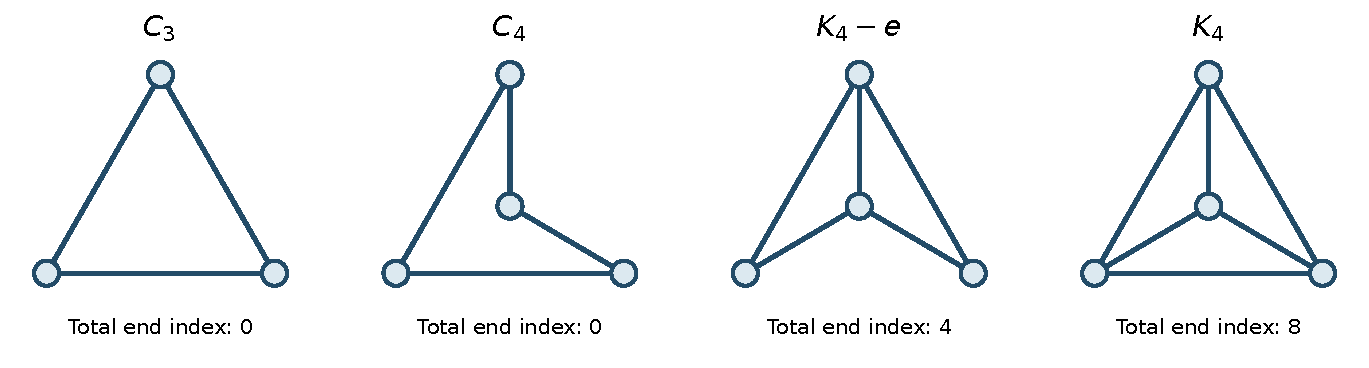
\includegraphics[width=\linewidth]{figures/local_characteristic_graphs.pdf}
\caption{The four possible nonempty local characteristic graphs in the
retained initial core.  Nodes are formal local face-port discs; edges are
surviving two-handle strips.  Every end has index zero or two.  The drawing
is a combinatorial schematic; the actual source embedding is retained in
the certificate.}
\label{fig:local-characteristic-graphs}
\end{figure}

\begin{theorem}[Initial admissibility with authenticated irreducibility]
\label{thm:unused-initial-compiler}
Given a finite triangulation of a compact connected orientable irreducible
three-manifold with one torus boundary and empty boundary pattern, the
incidence cancellations and unused-cocore quotient give, in polynomial
encoded time, either
\begin{enumerate}
 \item a solid-torus certificate from the first case of
 Corollary~\ref{cor:unused-torus}; or
 \item an inherited handle presentation, homeomorphic to the source,
 that is admissible for the empty pattern.
\end{enumerate}
The second output consists of the handles in the unique Euler-zero piece;
the source charts and cancellation trace retain their provenance.  No
normal surface search or boundary-period transport is required.
\end{theorem}

\begin{proof}
Termination and polynomial cost of the cancellation queues follow because
each move removes a handle pair and each attaching occurrence is removed
at most once.  The quotient and Euler counts are finite graph operations.
In the cycle case the preceding corollary gives the solid torus.

In the tree case cut all unused cocores and retain the unique Euler-zero
piece.  The other pieces are balls, and the corollary gives a homeomorphism
with the original manifold.  Every one-handle of the retained presentation
is used and hence has $d(e)\geq2$.  Each of its characteristic zero-handle
ends has index
\[
   -4+2d(e)\geq0.
\]
An index-zero end is disjoint from the pattern, because the pattern is empty.
For the second condition, Lemma~\ref{lem:unused-k4} shows that every
complementary region of the characteristic surface in a zero-handle
boundary is a disc.  A simple closed curve disjoint from the characteristic
surface therefore bounds a disc in that same complement, and the disc
meets the empty pattern in the empty set.  This proves the stronger
complement-disc condition, as well as the printed admissibility condition;
we do not rely on the weaker observation that an arbitrary sphere curve
bounds a disc that might contain characteristic handles.  Both required
conditions therefore hold.
\end{proof}

The retained core is a handle subpresentation, not a fresh triangulation.
It includes inherited source identifiers, its assigned two-handles, and
the geometric reduction trace.  This suffices to authenticate its unmarked
homeomorphism type and initial admissibility.  It does not provide an
explicit parametrization of every discarded ball, a transport map for an
arbitrary later pattern, or a normal-coordinate adapter on a retriangulated
core.  Those remain implementation tasks.

For an input knot diagram, the implementation's wrapper independently checks
that the supplied triangulation is the canonical exterior of that exact
classical one-component diagram.  A knot exterior in the three-sphere is
irreducible: a sphere disjoint from the connected knot bounds a ball on the
side not containing the knot.  Thus the wrapper authenticates the theorem's
hypothesis.  It returns \texttt{UNKNOT} in the cycle case and
\texttt{ADMISSIBLE\_CORE} in the tree case.  The latter is an intermediate
result, never a knottedness certificate.

\subsection{Why the irreducibility gate cannot be replaced by a flag}

The delivered exact controls \texttt{solid\_torus\_sum\_rp3} and
\texttt{solid\_torus\_sum\_s2xs1}, copied from the pinned source corpus,
are reducible manifolds with torus boundary.  Both produce $\beta=1$ with
Euler characteristic one for every cut piece.  An independent Regina
check finds that neither is a solid torus.  In particular, the quotient
and the Euler data alone do not distinguish the ball pieces from punctured
closed summands.

This has a direct classical model.  Let $N$ be a closed orientable
three-manifold other than the sphere, remove a ball, and take the boundary
connected sum of the resulting punctured manifold with a solid torus.
The result is the connected sum of the solid torus and $N$.  Cutting a
meridian cocore leaves a piece with Euler characteristic one, but the
punctured $N$ remains.  If $N=\mathbb{RP}^3$, its fundamental group already
precludes a ball.  If $N=S^2\times S^1$, the additional infinite-cyclic
free factor does the same.

The generic \texttt{verify\_unused\_handle\_certificate} therefore
authenticates only the geometric decomposition and its numerical case.
It never authorizes an irreducibility assertion from a caller's Boolean.
The diagram wrapper verifies exterior provenance first.  Mutating a valid
diagram certificate to substitute either reducible source is rejected.

\subsection{Linear replay of geometric cancellation traces}

The maintained independent cancellation checker reconstructs source cells
separately from the producer.  For each proposed one/two-handle cancellation
it scans every surviving two-handle attaching cycle to confirm that the
selected one-handle occurs once in total.  This is sound but can repeatedly
scan the same surviving rows.

\begin{proposition}[Occurrence-count replay]
\label{prop:unused-linear-replay}
After independently reconstructing the geometric attaching rows, a supplied
cancellation trace with $h$ handles and $L$ attaching occurrences can be
checked using $O(h+L)$ combinatorial incidence updates, excluding ordered
output construction and source reconstruction.  Its acceptance condition
for each one/two cancellation is identical to the full-scan condition.
\end{proposition}

\begin{proof}
Let $m_{ef}$ be the nonnegative number of occurrences of one-handle $f$
in the attaching circle of two-handle $e$.  Initialize
$d_f=\sum_{e\text{ alive}}m_{ef}$.  Deleting $e$ subtracts $m_{ef}$ from
$d_f$ for every nonzero entry of that row.  At a proposed cancellation
of $f$ with $e$, require both to be alive and require
\[
   d_f=1,\qquad m_{ef}=1.
\]
Since all multiplicities are nonnegative, these conditions say exactly
that $e$ supplies the unique geometric occurrence of $f$ among all alive
two-handles.  Signed cancellation plays no role.  The two/three-handle
condition is checked separately using the surviving endpoint occurrences,
and its deleted row is charged in exactly the same way.

Each row is deleted at most once.  Its incidence entries are visited once
at initialization and once at deletion.  The handle-state tests and final
counts use linear additional work.  An independently recomputed final
degree table can be checked in one further pass without changing the bound.
\end{proof}

The prototype uses union by size and path compression for the producer's
quotient, followed by canonical component numbering.  The verifier uses
breadth-first search on separately reconstructed raw source cells, without
calling the producer, its union-find routine, or its scheduler.  It also checks the local facet ports and source-edge strips in
Lemma~\ref{lem:unused-k4}, including their geometric degrees and local
connectedness.  The two paths share immutable input formats and elementary arithmetic; the source
geometry constructions are the established distinct maintained paths.

All source identifiers, degrees, and component sizes have $O(\log(t+1))$
bits.  The incidence and quotient certificates contain $O(t)$ records and
therefore occupy $O(t\log(t+1))$ bits.  Original source validation,
fingerprinting, and raw-cell reconstruction remain additional polynomial
costs.  The linear incidence theorem does not assert that the entire Python
source-validation stack has linear bit complexity.

\subsection{A proved certificate-size separation on Fibonacci layered tori}
\label{subsec:unused-fibonacci}

The standard layered-solid-torus fixture makes the eliminated boundary
arithmetic explicit.  Number its tetrahedra $0,\ldots,t-1$.  For
$i<t-1$, face zero of tetrahedron $i$ is paired to face two of $i+1$ by
the vertex permutation $(2,1,3,0)$, and face one is paired to face three
of $i+1$ by $(0,3,1,2)$.  In the last tetrahedron, face zero is paired to
face one by $(1,2,3,0)$.  Reverse pairings are the inverse permutations;
faces two and three of tetrahedron zero remain boundary.  This is the
maintained Fibonacci layered-solid-torus family, not a newly proposed
topological construction.

For $0\leq i\leq t-2$, write $a_i,b_i$ for the dual one-handles of face
zero and face one of tetrahedron $i$, and write $c$ for the final self-paired
handle.  Their native identifiers are $2i,2i+1,2t-2$, respectively.
Following the interior-edge links through the displayed face permutations
gives the attaching words
\begin{align}
 r_i&=b_i a_{i+1}a_{i+2}b_{i+2}^{-1}b_{i+1}^{-1}a_i^{-1}
     &&(0\leq i\leq t-4),\
 r_{t-3}&=b_{t-3}a_{t-2}c\,b_{t-2}^{-1}a_{t-3}^{-1},\
 r_{t-2}&=b_{t-2}c^2a_{t-2}^{-1}.
 \label{eq:unused-layered-relators}
\end{align}
The penultimate line is present for $t\geq3$, the last for $t\geq2$;
the case $t=1$ has only $c$ and no two-handle.  The first line is the
repeating six-sector link.  The final two lines are its five-sector and
four-sector closures at the self-paired end.  Here is an explicit check of
the three local types.  Write $(j,uv;p,q)$ for the sector at edge $uv$ in
tetrahedron $j$, entering through facet $p$ and leaving through facet $q$.
For $0\leq i\leq t-4$ the successive sectors are
\[
\begin{aligned}
 &(i,23;0,1)\longrightarrow(i+1,12;3,0)
     \longrightarrow(i+2,13;2,0)\\
 &\hspace{6mm}\longrightarrow(i+3,01;2,3)
     \longrightarrow(i+2,02;1,3)
     \longrightarrow(i+1,03;1,2).
\end{aligned}
\]
The last exit returns to the first entry.  At $i=t-3$, the self-pairing
replaces the middle step through tetrahedron $i+3$ by a direct passage
from $(i+2,13;2,0)$ to $(i+2,02;1,3)$, giving the five-sector word.
At $i=t-2$, the four sectors are
\[
 (i,23;0,1)\longrightarrow(i+1,12;3,0)
 \longrightarrow(i+1,23;1,0)
 \longrightarrow(i+1,03;1,2).
\]
Reading the exiting facet pairings gives exactly
\eqref{eq:unused-layered-relators}, including two successive positive
crossings of $c$ in the last case.  The calculation uses only the displayed
face permutations, so it proves the words for every $t$.

\begin{proposition}[Fibonacci transport and certificate separation]
\label{prop:unused-fibonacci-separation}
For this family, the maintained queue cancels $(a_i,r_i)$ in the order
$i=0,\ldots,t-2$.  Its remaining one-handles are $b_0,\ldots,b_{t-2},c$.
The native transported cocycle for the surviving cocore $c$ has
\begin{equation}
  x(b_i)=0,\qquad x(c)=1,\qquad x(a_i)=F_{t-i+1}.
  \label{eq:unused-fibonacci-values}
\end{equation}
Consequently, the native explicit dual-value list alone occupies
$\Theta(t^2)$ binary bits.  The new source incidence/component certificate
occupies $O(t\log(t+1))$ bits and contains no transported cocycle.
\end{proposition}

\begin{proof}
Initially $a_0$ occurs exactly once.  After rows $r_0,\ldots,r_{i-1}$
are removed, $a_i$ occurs exactly once in $r_i$.  The native queue places
$a_i$ before $b_i$: in the row whose removal first makes them unique,
the occurrence of $a_i$ precedes that of $b_i$.  Once $a_i$ is cancelled,
the pending $b_i$ has degree zero and is skipped.  Future $a_j$ have more
than one occurrence until this step, and $c$ retains its double occurrence
in the final row.  This proves the stated cancellation order and remainder.

The remaining $b_i$ form a tree joining the $t$ zero-handles, while $c$
is its single additional loop.  The surviving-cocore assignment sets all
$b_i$ to zero and $c$ to one.  Reading the final two equations in
\eqref{eq:unused-layered-relators} gives
\[
 x(a_{t-2})=2,\qquad x(a_{t-3})=3.
\]
Every preceding row gives
\[
 x(a_i)=x(a_{i+1})+x(a_{i+2}).
\]
Uniqueness of reverse substitution proves \eqref{eq:unused-fibonacci-values},
including the two small end cases.

The $t$ nonzero values are $F_2,F_3,\ldots,F_{t+1}$.  The recurrence gives
$F_{j+2}\geq2F_j$ and $F_j\leq2^{j-1}$, so
$\log_2 F_j=\Theta(j)$.  Summing their individual bit lengths proves the
quadratic bound.  In the new quotient every $K_i$ is just one zero-handle,
$Q$ has $t$ edges and $t$ vertices, and the trace has $t-1$ cancellations.
All identifiers are bounded by a constant multiple of $t$, proving the
new upper bound.
\end{proof}

This is a comparison with the maintained explicit coordinate-list
certificate, not a lower bound on every possible cocycle encoding.  A
recurrence-based encoding could also compress those Fibonacci integers.
The new certificate avoids constructing and checking them at all because
the authenticated geometric situation supplies a different proof.
For general input diagrams the second branch of
Theorem~\ref{thm:unused-initial-compiler} may remain, so this size separation
does not prove completeness of a polynomial unknot-recognition method.

\subsection{Finite verification and performance scope}

The delivered tests replay all 48 supplied source triangulations and compare
the new cancellation sequence, remaining handle sets, summary, and source
fingerprint with the maintained implementation.  The same incidence-only
certificates also pass the unchanged maintained cancellation verifier.
Additional checks cover 48 independent local/global relabellings, canonical
diagram exteriors, forged component lists and cycle ranks, Boolean labels,
wrong diagram provenance, caps, cooperative interruption, and the two
reducible controls.  The replay tests disable the producer routines to
confirm the independent call path.  An optional Regina oracle supplies
separate solid-torus and nonball checks.

There is also an unbounded geometric ballast family.  Attach a chain of
tetrahedral balls to embedded boundary triangles of the canonical trefoil
exterior.  The first triangle has three distinct quotient vertices, and
each next one contains two old vertices and the new vertex, so each
attachment is an elementary boundary shelling.  A reverse-shelling checker
authenticates the family.  Each extra tetrahedron contributes one ball
component and one unused bridge, while the retained torus core is unchanged.
The source packet therefore removes arbitrarily many irrelevant handles
without any claim that the irreducible core itself has bounded complexity.

\begin{table}[htbp]
\centering\small
\begin{tabular}{lrrrrr}
\hline
Source & $t$ & Native ms & New ms & Native/New & Core $h_0$ \\
\hline
Fibonacci $t=1$ & 1 & 0.473 & 0.458 & 1.034 & --- \\
Fibonacci $t=16$ & 16 & 6.250 & 6.180 & 1.011 & --- \\
Fibonacci $t=64$ & 64 & 22.753 & 21.435 & 1.061 & --- \\
Fibonacci $t=256$ & 256 & 173.290 & 159.682 & 1.085 & --- \\
Fibonacci $t=512$ & 512 & 667.727 & 578.314 & 1.155 & --- \\
Canonical unknot & 40 & 11.925 & 11.690 & 1.020 & --- \\
Canonical trefoil & 60 & 19.005 & 20.213 & 0.940 & 48 \\
Canonical figure-eight & 80 & 29.950 & 28.445 & 1.053 & 68 \\
Trefoil + 32 buds & 92 & 30.324 & 29.663 & 1.022 & 48 \\
Trefoil + 256 buds & 316 & 108.484 & 117.183 & 0.926 & 48 \\
\hline
\end{tabular}
\caption{5 paired repetitions per source, in randomized order. Values are medians of complete producer-plus-replay times. Ratios below one are regressions. A dash marks the all-ball cycle branch.}
\label{tab:unused-timings}
\end{table}

\begin{table}[htbp]
\centering\small
\begin{tabular}{rrrrr}
\hline
Fibonacci $t$ & Native bytes & New bytes & Max. dual bits & Sum dual bits \\
\hline
1 & 581 & 699 & 1 & 1 \\
16 & 2441 & 4010 & 11 & 111 \\
64 & 9787 & 14865 & 44 & 1510 \\
256 & 58924 & 59551 & 178 & 23103 \\
512 & 172549 & 119503 & 355 & 91702 \\
\hline
\end{tabular}
\caption{Exact compact-JSON sizes and bit counts. The new decomposition has additional per-component records, so its asymptotic improvement need not appear at small sizes. Total dual bits includes one bit for each zero entry.}
\label{tab:unused-bits}
\end{table}

The canonical trefoil core retains $(h_0,h_1,h_2)=(48,82,34)$ from a source with 60 tetrahedra; the figure-eight core retains $(68,118,50)$ from 80 tetrahedra. Every added boundary bud leaves the trefoil core unchanged. At $t=512$, the new Fibonacci certificate uses 119,503 bytes versus 172,549 bytes for the maintained certificate; at $t=64$, it instead uses 14,865 versus 9,787 bytes. These finite measurements agree with the scope, and the crossover limitations, of Proposition~\ref{prop:unused-fibonacci-separation}. Timing regressions on some sources remain visible; the source-validation and raw-cell construction costs are included in both arms.


The benchmark measures completed source producer plus independent replay,
with randomized paired order and all raw repetitions retained.  It excludes
serialization and canonical-diagram construction.  The old query emits
the geometric reduction and, on a hit, its transported boundary period;
the new query emits the geometric reduction and the exact cut decomposition.
Their source outputs differ, and the new topological interpretation uses
separately authenticated irreducibility.  These are source-operator
measurements, not whole-recognizer timings.  The maintained recognition
defaults are unchanged and no new knot coverage is asserted.

\section{A source-authenticated native moment compiler}
\label{sec:native-moments}

The incoming moment construction left its passage from the maintained
parallelity geometry to a weighted first-return query as a separate task.
We implement that passage here.  The resulting operator starts with an
actual triangulation and binary normal coordinates, or with the complete
parallelity certificate for that source.  It produces the same cyclic
core-port words and attachment components as the maintained native boundary
compiler, and adds the exact number of original-boundary edges in every
complementary gap.

The maintained operator uses two scalar weighted censuses: one to identify
marked corners, and one on the fibre double cover to identify residual
gaps and their fibre transport.  The new operator performs one scalar
census on that same residual double cover.  It replaces the corner query
by canonically owned edge mass, and replaces the lifted endpoint masks by
quadratic moments.  These are improvements to an existing geometric
operation.  They do not supply a new cutting surface or establish a
uniform bound on the number of stages in a recognition hierarchy.

\subsection{The actual native packet}

Fix a source with $T$ tetrahedra and an accepted normal-coordinate vector.
Let $G$ be its compressed parallelity geometry at the audited source
revision.  A polygon family $P$ has a binary rank interval and a distinct
corner-occurrence interval for every corner of its polygon template.
Write $c_{P,j}$ for the start of the interval at corner $j$.  The occurrence
of corner $j$ at rank $k$ has coordinate
\[
                 x(P,j,k)=c_{P,j}+k-1.
\]
The entire corner namespace is $X=\{0,\ldots,N-1\}$.  Its size $N$ can be
exponential in the bit length of a normal multiplicity.  No construction
below enumerates $X$.

The packet contains a list of polygon-edge gluings.  Such a gluing has
affine rank maps of slope $1$ or $-1$, an endpoint-reversal flag, and a
separate fibre-reversal flag.  The latter cannot be recovered from the
slope of a singleton rank interval.  The packet also gives a disjoint
inventory of unglued polygon-edge occurrences.  Each inventory record is
either an original-boundary family or one singleton core-facing edge,
called a \emph{port}.  Ports have distinct identifiers $0,\ldots,p-1$ and
the supplied ordering of their two local endpoints.  The source construction
has $p\leq66T$.

The geometric correctness of the source packet entails that its free edges,
after corner identifications, form cellulated boundary circles.  A circle
may have only one edge; its two incidence flags are still distinct.  The
fibre labels define a genuine interval bundle over these circles and their
corner stars.  The reference source reconstruction in the checker is
independent of the production geometry builder.  Consequently the new
checker does not accept a purported degree-two boundary merely because its
moment histogram happens to look plausible.

\begin{lemma}[Native canonical ownership]
\label{lem:native-edge-ownership}
For an original-boundary record on edge $j$ of polygon family $P$, with
rank interval $[u,v)$, place unit edge mass on the interval
\[
                 [c_{P,j}+u-1,c_{P,j}+v-1)\subset X.
\]
This assigns every original-boundary edge exactly one owner occurrence,
and the owner represents one endpoint of that edge.  The owner intervals
of distinct original-boundary records are disjoint in $X$.  In particular,
if $E$ is the represented number of original-boundary edges, then
$E+p\leq N$.
For $a$ original-boundary records the ownership program has $a$ intervals,
irrespective of the binary lengths of those intervals.
\end{lemma}

\begin{proof}
At fixed $P,j$, the inventory records are the disjoint rank gaps remaining
after the explicitly recorded edge gluings; they cannot contain the same
rank twice.  The map $k\mapsto c_{P,j}+k-1$ is injective.  Different corner
slots and different polygon families have disjoint occurrence namespaces
by the construction of the $c_{P,j}$.  Thus all the indicated intervals
are disjoint.  Their lengths are precisely the numbers of represented
edge occurrences.  Each recorded free edge belongs to this inventory once,
so summing the lengths counts each original-boundary edge exactly once.
The chosen corner is its local initial endpoint.  Identifying corner
aliases later does not change this count: several owners can become one
actual vertex, and their masses are added there.  Apply the same outgoing-corner assignment also to the $p$ port singletons.
They remain disjoint from each other and from the original-boundary
intervals, because the complete free-edge inventory is disjoint.  These
intervals have total length $E+p$ and lie in a namespace of size $N$,
proving $E+p\leq N$.
\end{proof}

\subsection{Compiling the residual fibre cover}

Delete all open port edges.  The remaining boundary is a union of compact
paths, passive circles, and possibly silent occurrence classes that never
meet a free edge.  The source relation for the residual paths is generated
by the corner gluings and by the endpoint identifications of all
original-boundary edges.

To retain local fibre transport, replace $X$ by
$\widetilde X=X\times\{0,1\}$, encoded as $x+sN$.  A source corner gluing
with fibre flag $f$ joins sheet $s$ to sheet $s\mathbin{\oplus}f$.
An original-boundary edge joins its endpoints on the same local sheet.
Every source interval pairing therefore creates a bounded number of
affine interval pairings in $\widetilde X$.

\begin{lemma}[Residual degree and exact length]
\label{lem:native-residual-degree}
If $p>0$, the residual components meeting port endpoints are exactly $p$
paths, counting a point as a path of length zero.  Each has two distinct
endpoint occurrences, and has two lifts to the fibre cover.  A lifted
residual component contains precisely two lifted endpoint labels.
Its canonically owned edge mass equals the number of original-boundary
edges of the underlying path.  This number is zero if and only if the two
port endpoints represent the same actual corner.
\end{lemma}

\begin{proof}
A boundary circle containing $q>0$ distinct ports becomes $q$ compact
intervals when their open interiors are removed.  Consecutive port edges
can meet at one vertex, giving a point interval.  If the entire circle
consists of one port edge, deleting its interior gives one point with two
distinct endpoint occurrences.  Summing over active circles gives $p$
residual paths.

An interval bundle restricted to a contractible path is a product, so the
corresponding two-sheeted fibre-orientation cover has two path components.
Each contains one lift of each endpoint occurrence.  Every edge owner
belongs to the same residual class as the endpoints of its edge.  By
Lemma~\ref{lem:native-edge-ownership}, no edge contributes twice, and no
edge outside the path contributes to it.  Lift the ownership program once
on each sheet.  Each lifted path therefore receives exactly its underlying
edge count.  A finite cellulated interval has equal endpoint vertices
precisely when it is a point.  Positive length cannot return to its initial
vertex within a genuine degree-two residual boundary containing a port.
Passive circles and silent interior classes carry no endpoint labels.
\end{proof}

The last equivalence is where source geometry matters.  In an arbitrary
quotient graph a positive-length cycle can have the same initial and final
vertex.  The scalar moment data alone do not exclude that situation.

\subsection{The four-field reference codec}

The implementation retains the incoming four-field construction as
\texttt{codec='four'} for differential verification.  For $p>0$ there
are $r=4p$ lifted terminal labels.  Port $j$, local endpoint
$e\in\{0,1\}$, and local fibre sheet $s\in\{0,1\}$ receive the distinct
label
\[
                       i=4j+2e+s+1.
\]
Define
\begin{equation}
\label{eq:native-moment-base}
 S_2=\frac{r(r+1)(2r+1)}6,
 \qquad h=\operatorname{bitlength}(S_2),
 \qquad \beta=2^h.
\end{equation}
The terminal label $i$ contributes
\begin{equation}
\label{eq:native-terminal-scalar}
                         1+i\beta+i^2\beta^2
\end{equation}
at its lifted corner occurrence.  Every lifted owner edge contributes
$\beta^3$.  Contributions at the same occurrence are added.  Both terminal
and ownership contributions are supplied as additive constant-weight
intervals to the maintained weighted-orbit API.

The global terminal count, global first moment, and global second moment
are all strictly less than $\beta$.  Hence no carry between the three
lower fields is possible, even before one uses the degree-two property.
For an orbit of scalar weight $w$ successive divisions by $\beta$ give
\[
               w=t+\beta u+\beta^2 v+\beta^3\ell,
               \qquad 0\leq t,u,v<\beta.
\]
If $t>0$, Lemma~\ref{lem:native-residual-degree} gives $t=2$ and labels
\begin{equation}
\label{eq:native-moment-decode}
 d=\sqrt{2v-u^2},\qquad
 i=\frac{u-d}{2},\qquad j=\frac{u+d}{2}.
\end{equation}
The decoder uses an exact integer square root.  It checks a positive square
discriminant, parity, label range, unique label usage, and coverage of all
$r$ labels.  A terminal-bearing histogram row must have orbit multiplicity
one, because the same globally unique pair of labels cannot belong to two
different orbits.  A terminal-free row is ignored only after its lower
three fields have been checked to be zero.

\subsection{A smaller codec using the native degree-two structure}

The default \texttt{codec='pair'} exploits the authenticated native
boundary contract more closely.  Once residual degree two is known, no
explicit count field is needed to recover a pair.  Moreover, the scalar
radices can be chosen using the maximum mass of two labels on one path,
instead of the sums of all labels in the entire namespace.  This improves
the power of $p$ in the scalar-magnitude bound from nine to three.

Put
\begin{equation}
\label{eq:native-pair-codec}
 A=2^{\operatorname{bitlength}(2r)},\qquad
 s_i=i+A i^2,\qquad
 D=2^{\operatorname{bitlength}(2(r+A r^2))}.
\end{equation}
The terminal label $i$ contributes $s_i$ and every lifted owner edge
contributes $D$.  Both radices are powers of two, so the implementation
uses integer shifts and masks.

\begin{lemma}[Path-local no-carry decoding]
\label{lem:native-pair-packing}
For a lifted residual path with endpoint labels $i<j$ and edge length
$\ell$, its scalar orbit weight is
\[
                        W=\ell D+s_i+s_j.
\]
It determines the endpoint pair and length by
\begin{equation}
\label{eq:native-pair-decode}
 \ell=\left\lfloor W/D\right\rfloor,\quad
 R=W\bmod D,\quad S=R\bmod A,\quad Q=\lfloor R/A\rfloor,
 \quad i,j=\frac{S\mp\sqrt{2Q-S^2}}2.
\end{equation}
The remainder is positive on every active lifted path and is zero on
every terminal-free orbit.
\end{lemma}

\begin{proof}
The source degree-two theorem supplies exactly two distinct labels on
each lifted active path.  Equation~\eqref{eq:native-pair-codec} gives
$A>2r\geq i+j$ and $D>2(r+A r^2)\geq s_i+s_j>0$.
Consequently neither radix receives a carry from the fields beneath it:
$R=s_i+s_j$, $S=i+j$ and $Q=i^2+j^2$.  The quadratic identity
$2Q-S^2=(j-i)^2$ proves the decoder.  Terminal-free orbits consist only of
edge mass, which is an integer multiple of $D$.  Nonnegative edge mass
and positive terminal labels rule out cancellation.
\end{proof}

This is a path-local radix proof.  The sum of terminal weights over the
whole namespace need not be smaller than $D$, and the implementation
never assumes that it is.  The checker still requires multiplicity one
on active histogram rows, exact positive square discriminants, admissible
roots, full label coverage, consistent deck-paired lifts and equal lengths
on the two lifts.  The source geometry, query weights and orbit proof are
independently authenticated before the decoded words are accepted.  The
smaller codec does not furnish a degree-two geometric-boundary certificate
for an arbitrary quotient graph.

There is nevertheless a useful stronger arithmetic safeguard.  Completeness
of the recovered matching, together with the known input label inventory,
replaces the explicit occupancy coordinate even when one does not assume
degree two in advance.

\begin{lemma}[Global inventory forces pair occupancy]
\label{lem:native-pair-global-inventory}
Consider an arbitrary equivalence relation on a finite occurrence namespace.
Each of the $r$ distinct positive labels occurs exactly once, with scalar
weight $s_i$ from~\eqref{eq:native-pair-codec}; all other weight contributions
are nonnegative integer multiples of $D$.  Suppose a complete, exact
weighted orbit histogram passes the following arithmetic checks:
\begin{enumerate}
  \item every row of nonzero remainder modulo $D$ has orbit multiplicity
  one and decodes to two distinct roots in $\{1,\ldots,r\}$;
  \item the decoded pairs are disjoint and exhaust this label set.
\end{enumerate}
Then every orbit containing labels contains exactly two of them, no
label-containing orbit has zero remainder, and every decoded pair is its
actual pair of labels.  If $H$ is the sum of its nonterminal scalar
contributions, its decoded quotient satisfies $\lfloor W/D\rfloor=H/D$.
\end{lemma}

\begin{proof}
An orbit with no labels has zero remainder modulo $D$.  An orbit with only
label $i$ has remainder $s_i$, since $0<s_i<D$.  Since $i<A$, its decoded
moment coordinates are $S=i$ and $Q=i^2$, whose quadratic roots are $0,i$.
Such a row cannot pass the requirement of two positive roots.  Hence every
accepted nonzero row represents one actual orbit containing at least two
labels.

The exhaustive disjoint decoded inventory contains exactly $r/2$ pairs.
Their $r/2$ actual orbits therefore consume at least $r$ actual labels.
There are precisely $r$ labels in the whole input, counted once each.
Equality follows: every accepted row contains exactly two labels, and no
labels remain in a row of zero remainder or in any other orbit.  Now the
path-local arithmetic inequalities used in
Lemma~\ref{lem:native-pair-packing}, which depend only on having two labels,
apply to every accepted row.  They recover its actual two labels and the
sum of the integer coefficients of $D$ in its nonterminal contributions.
\end{proof}

The complete authenticated histogram and the exact initial inventory are
essential to this argument.  Local moment roots alone are insufficient:
the three labels $\{1,2,6\}$ have the same first two moments as the pair
$\{4,5\}$.  The global argument excludes such a row in a complete accepted
partition by counting actual label consumption.  This is an arithmetic
soundness statement.  It does not turn a two-label orbit in a branched
graph into a geometric interval, or prove that its arbitrary mass counts
genuine boundary edges.  Those conclusions still require the independently
verified source geometry and canonical ownership theorem.

\begin{theorem}[Native first-return bridge]
\label{thm:native-moment-bridge}
For a valid authenticated native parallelity packet with $p>0$ ports,
one scalar weighted orbit histogram on $\widetilde X$ determines:
\begin{enumerate}
  \item the first-return matching of all $2p$ base endpoint occurrences;
  \item the local fibre reversal and the exact original-boundary edge
  length of each matched gap;
  \item the signed cyclic port words, their gap order, and the decomposition
  of the core attachment into proper intervals and whole boundary circles.
\end{enumerate}
After forgetting the newly added edge lengths, the output equals the
maintained native boundary-word output, with the same canonical port
ordering and local chart convention.  No separate corner census is needed.
For $p=0$ the cyclic interface is empty and no new census is performed.
\end{theorem}

\begin{proof}
Use either the four-field decoder~\eqref{eq:native-moment-decode} or
the default decoder~\eqref{eq:native-pair-decode} to obtain the perfect
matching on lifted labels.  For a base endpoint $a$, write the mate of its sheet-zero
lift as $2b+f$, now using zero-based lifted labels.  The mate of its other
lift is $2b+(1-f)$.  These two relations recover the base mate $b$ and fibre
flag $f$.  The two lifted path lengths agree, and the implementation checks
this equality explicitly.  It also checks $b\ne a$ at the level of
endpoint occurrences; actual corner equality remains allowed.

By Lemma~\ref{lem:native-residual-degree}, zero length means the two ends
share a corner, and positive length means original boundary is present.
These are exactly the data recovered by the maintained compiler's separate
corner query and lifted endpoint-mask query.  To recover cyclic order,
cross a port and then its following matched gap.  This permutation on
oriented endpoint occurrences traverses each active boundary circle in
one of its two directions.  Start with the least unused port in its
positive local chart, matching the maintained convention.  Every port
appears once.  The parity of the gap fibre flags around a complete circle
must be zero; this is checked rather than inferred from rank slopes.

If every gap in a word has length zero, the attachment is the whole circle.
Otherwise, begin immediately after every positive-length gap and collect
successive ports across zero-length gaps.  These maximal runs are exactly
the proper interval attachments.  Their endpoint tokens and fibre parity
are read from the same matching and ordered gap flags.  Thus all fields of
the existing skeleton are identical, while the new positive integer
lengths refine its original-boundary-present booleans.  Neither traversal
requires reconstructing endpoint masks.  The case $p=0$ is immediate.
\end{proof}

\paragraph{What the local charts do not provide.}
The chosen direction on each word is a canonical reporting convention.
It is not a coherent boundary orientation of all the circles belonging to
one orientable base.  The native packet supplies local port charts and
fibre transitions; a later surgery algorithm requiring coherent base
frames must derive or receive those frames separately.  Similarly, the
word does not retain an arbitrary additional boundary marking lying
inside a positive-length gap.

\subsection{Encoded cost and the actual implementation claim}

\begin{proposition}[Input scalar and output-size bounds]
\label{prop:native-moment-size}
For the default pair codec with $p>0$, every additive input weight has
$O(\log(p+1))$ bits.  Its total scalar mass on the double cover is less
than
\begin{equation}
\label{eq:native-total-mass}
             2(E+p)D\leq2ND=O\bigl(N(p+1)^3\bigr).
\end{equation}
Every active orbit separately has scalar weight less than $(N+1)D$.
Consequently every orbit weight uses
$O(\log(N+1)+\log(p+1))$ bits, with only three logarithmic powers of $p$
in the scalar bound.  The gap and word portion of the returned cyclic
interface uses
\[
                  O\bigl(p(\log(N+1)+\log(p+1))\bigr)
\]
bits.  The complete skeleton also carries source core-handle identifiers;
its bound is $O(p(\log(N+1)+\log(T+1)+\log(p+1)))$, excluding discovery
certificates and the optional base-profile ledger.  Its assembly uses
$O(p)$ endpoint and gap records and never materializes an $O(p)$-bit
incidence mask.
\end{proposition}

\begin{proof}
Equation~\eqref{eq:native-pair-codec} gives $2r<A\leq4r$ and
\[
   2(r+A r^2)<D\leq4(r+A r^2)\leq20r^3.
\]
Every terminal contribution satisfies $s_i<D/2$.  There are $r=4p$
terminal contributions and $2E$ lifted owner edges.  The total scalar
mass is therefore less than
\[
                    2ED+(r/2)D=2(E+p)D\leq2ND.
\]
An active orbit has at most $E$ owner edges and terminal remainder less
than $D$, giving the stated per-orbit bound.  These inequalities also
bound the input scalar bit lengths.

There are $p$ gaps, each with two endpoint identifiers, one fibre bit and
one length at most $E$.  The cyclic words contain $p$ port occurrences in
total.  The attachment words also contain each port once, so their total
length is $p$.  Source port ranks have $O(\log(N+1))$ bits, while the
source core-handle identifiers have $O(\log(T+1))$ bits.  These facts give
the two output bounds.  The latter term cannot be discarded merely because
only a few tetrahedra contain nonzero normal coordinates.  The direct
matching and successor traversals need only a bounded number of arrays
or dictionaries indexed by the $O(p)$ endpoints and gaps.
\end{proof}

For comparison, the retained four-field codec has
$\beta\leq2r^3$ and total scalar mass less than
$(2E+1)\beta^3=O((N+1)(p+1)^9)$.  Both encodings have the same big-O
binary length, but the path-local codec reduces the number of label bits
and scalar-arithmetic constants.  The complete decoded outputs agree.

If there are $g$ source gluing records and $a$ original-boundary free-edge
records, the double-cover query has $4g+2a$ pairing records and $4p+2a$
additive weight records.  A simple endpoint sweep initially canonicalizes
these additions into $O(a+p)$ weight runs.  The source construction makes
$g+a+p=O(T)$, with binary endpoints.  Exact length extraction therefore
preserves the polynomial encoded size of the source query.

There is a practical tradeoff.  The maintained sparse-mask compiler has
input weights only at marked endpoints; its previously established
uniform sparse-token run bound does not apply to the new edge-mass query.
Original-boundary owner intervals add weight runs.  The initial bound is
$O(a+p)$, not a port-only bound, and the measured maximum number of runs
can be larger even though one entire census has been removed.

The weighted Agol--Hass--Thurston theorem supplies a polynomial algorithm
for the encoded weighted interval-orbit task
\cite[Theorem~16]{AgolHassThurston2006}.  Composing that theorem with the
explicit reduction above gives a polynomial bound for this native
first-return problem in the source record count and binary lengths.  This
is an algorithmic existence and reduction statement.  We do not infer a
new uniform polynomial bound on every intermediate weight run or every
certificate trace of the particular maintained Python implementation.
For that implementation the package supplies independently replayed
executions, cancellation contracts, and concrete measurements.  Those
executions are evidence about the implementation; they are not a proof of
its uniform worst-case trace complexity.

\subsection{Certificates, owner profiles, and failure contracts}

The direct API is \texttt{normal\_parallelity\_moment\_words}.
Its certificate binds the selected codec and contains the source
fingerprint, the complete cyclic
skeleton and one weighted census certificate.  The checker reconstructs
the geometry through the maintained raw-cut reference path, independently
builds the lifted affine pairings and ownership weights, replays the
weighted trace, decodes the moment pairs by a separate implementation,
and reconstructs the words using a separate permutation traversal.  It
imports neither the new producer nor its query builder, decoder or
assembly routine.  Tests disable those functions, both native discovery
schedulers, and the production geometry builder while the checker replays
a serialized binary certificate.

The optional \texttt{moments\_from\_parallelity\_packet} API accepts an
existing full normal-cut parallelity certificate.  It first verifies that
packet, including its four inherited discovery traces, then compiles one
new moment census from its authenticated free-edge inventory.  Source
authentication is additional work; it is not hidden in the one-new-census
claim.  Its combined certificate retains the upstream proof and binds
every active loop to its certified base-profile owner.  For a profile with
boundary count $b$ and $k$ active loops, the passive count is $b-k$.
Port-bearing profiles have multiplicity one; port-free profiles retain
their binary multiplicity and passive count per copy.  In this way even
passive components absent from the terminal census are preserved.

Discovery exhaustion returns \texttt{INCONCLUSIVE} without a skeleton or
certificate.  The direct replay cap counts its one trace; the packet
replay cap counts the sum of the four inherited traces and the new trace.
Malformed proofs return false, whereas cooperative cancellation and
invalid-source exceptions propagate.  These statuses are not knot
verdicts.  The new proof authenticates a compressed boundary operation,
not the validity or completeness of a proposed recognition hierarchy.

\subsection{Native verification and paired measurements}
\label{subsec:native-moment-measurements}

% BEGIN NATIVE MOMENT MEASUREMENTS
The verification passed eight native test groups in 113.590 seconds and
one additional arithmetic test group in 0.026 seconds.  Complete cyclic
outputs were compared on all 157 inherited source cases among the existing
native compiler and both new codecs.  Each new certificate was independently
replayed.  The edge-by-edge oracle could expand 146 of these cases; it
checked 219 positive-length gaps and 3420 point gaps.  The bank includes
five sources whose parallelity polygons are exclusively edge caps,
181 whole-circle attachment components, and 546 gaps with nontrivial local
fibre transport.  Additional cases cover layered-source multiples,
one-sided bases, source-packet authentication and JSON transport, altered
moments and lengths, source mismatch, exact resource caps and cancellation.

The arithmetic test enumerates all 4140 set partitions of eight terminal
labels, adds arbitrary nonnegative edge masses and silent repeated orbits,
and applies the no-count decoder.  It accepts exactly the 105 perfect
matchings and recovers their true pairs and masses.  All partitions
containing a singleton or an overfull terminal class are rejected.  This
is a finite regression check of
Lemma~\ref{lem:native-pair-global-inventory}, independent of the geometric
source-bank coverage.

For the $T=2$ layered source scaled by $m=2^b$, with
$b=32,512,16384$, the new census retained two ports, 60 lifted ownership
intervals, 68 additive weight records and 131 orbit cycles in every case.
This checks binary-coordinate handling without expansion.  The active
lengths in this family are both seven; the test is not presented as a
family of growing active gap lengths.  The unscaled $T=16$ source does
have a gap of 39787 edges, recovered without following them individually.

Table~\ref{tab:native-moment-times} reports five measurements per
implementation after one untimed warmup per implementation and source.
The execution order alternates existing--pair--four and
four--pair--existing.  Every timed discovery call starts with the original
triangulation and coordinates and includes source validation, geometry
construction, both or one orbit census respectively, complete cyclic
assembly and certificate construction.  No source geometry or orbit result
is reused.  The independent source-bound replay is timed separately.
These are local measurements on Python 3.12.14 under Linux x86-64 in the
shared execution environment, not hardware-isolated estimates or whole-knot
recognition benchmarks.

\begin{table}[H]
\centering\small
\setlength{\tabcolsep}{3pt}
\begin{tabular}{lrrrrrrr}
\toprule
& & \multicolumn{3}{c}{Discovery, ms} & \multicolumn{3}{c}{Replay, ms}\\
Case & $p$ & Existing & Four & Pair & Existing & Four & Pair\\
\midrule
Layered $T=2$ & 2 & 2.805 & 3.016 & 2.968 & 2.900 & 3.254 & 3.033 \\
Layered $T=4$ & 15 & 69.697 & 67.925 & 70.650 & 50.308 & 63.959 & 62.811 \\
Layered $T=8$ & 47 & 589.207 & 531.740 & 521.412 & 418.031 & 406.742 & 439.730 \\
Layered $T=16$ & 111 & 3754.319 & 3034.441 & 3057.760 & 2505.085 & 2278.534 & 2212.595 \\
$T=2$, $m=2^{32}$ & 2 & 40.726 & 36.990 & 33.990 & 20.270 & 28.035 & 29.060 \\
$T=2$, $m=2^{512}$ & 2 & 34.477 & 33.111 & 33.310 & 16.373 & 25.984 & 26.983 \\
$T=2$, $m=2^{16384}$ & 2 & 135.094 & 118.898 & 117.586 & 64.402 & 89.302 & 85.802 \\
Cap-only source & 8 & 0.454 & 0.434 & 0.461 & 2.007 & 1.726 & 1.686 \\
Port-free binary & 0 & 0.318 & 0.276 & 0.280 & 0.976 & 0.980 & 0.894 \\
\bottomrule
\end{tabular}
\caption{Median complete source-query and independent replay times.
Four denotes the reference four-field codec and Pair the default path-local
codec.  Both new codecs also certify exact gap lengths.}
\label{tab:native-moment-times}
\end{table}

\begin{table}[H]
\centering\small
\setlength{\tabcolsep}{4pt}
\begin{tabular}{lrrrr}
\toprule
Case & Orbit cycles & Peak runs & Scalar bits & Certificate KiB\\
\midrule
Layered $T=2$ & $42\to 37$ & $13\to 21$ & $25\to 14$ & $5.8\to 5.2$ \\
Layered $T=4$ & $250\to 189$ & $77\to 161$ & $52\to 21$ & $45.9\to 37.3$ \\
Layered $T=8$ & $690\to 485$ & $265\to 357$ & $67\to 27$ & $160.7\to 113.7$ \\
Layered $T=16$ & $1570\to 1077$ & $649\to 741$ & $76\to 30$ & $436.3\to 280.3$ \\
$T=2$, $m=2^{32}$ & $168\to 131$ & $17\to 85$ & $25\to 14$ & $37.5\to 31.8$ \\
$T=2$, $m=2^{512}$ & $168\to 131$ & $17\to 85$ & $25\to 14$ & $192.9\to 164.5$ \\
$T=2$, $m=2^{16384}$ & $168\to 131$ & $17\to 85$ & $25\to 14$ & $4435.1\to 3782.4$ \\
Cap-only source & $2\to 1$ & $16\to 16$ & $39\to 18$ & $3.1\to 2.7$ \\
Port-free binary & $0\to 0$ & $0\to 0$ & -- & $0.3\to 0.3$ \\
\bottomrule
\end{tabular}
\caption{Existing-to-pair structural measurements, except Scalar bits,
which compares the maximum additive input-weight bit length for
four-field versus pair codecs.  Orbit cycles sum the two existing censuses;
Peak runs takes their maximum.  Certificate size is compact JSON, using
hexadecimal transport for sufficiently large integers.  These are observed
sizes, not uniform worst-case bounds.}
\label{tab:native-moment-structure}
\end{table}

Compared with the existing native compiler, pair-codec discovery is about
$1.13$ times faster for $T=8$ and $1.23$ times faster for $T=16$ in this run.
The $T=2$, $T=4$ and cap-only examples are slightly slower.  Replay is not
uniformly faster: on the $m=2^{512}$ example it increases from 16.373 to
26.983 ms, whereas on the $T=16$ example it decreases from 2505.085 to
2212.595 ms.  The new ownership weights increase the maximum run count,
especially in the binary two-port family, from 17 to 85.

The pair codec reduces the maximum additive scalar from 76 to 30 bits
on the 111-port example and from 25 to 14 bits on the two-port binary
family.  Its wall-clock differences relative to the four-field codec are
small and mixed, as the table records.  Its principal justification is the
proved cubic scalar bound and the removal of the unnecessary count field;
a further uniform practical speedup is not claimed.  The complete single
samples, proof sizes and representative replayable certificates are
included in the results directory.
% END NATIVE MOMENT MEASUREMENTS

The native source bank contains shared-corner point gaps and whole-circle
attachments, but none of its explicitly expanded examples has a one-edge
boundary loop.  A separate geometric regression therefore tests a triangle
whose first two edges are identified in reverse, leaving its third edge as
a one-edge boundary circle.  Marking that edge must give one zero-length
gap and one circle attachment.  That test exercises the actual native
moment query and weighted proof replay, compared with a literal incidence
walk.  It is explicitly a geometric packet regression, not an additional
authenticated source triangulation.

The files \texttt{native\_moments.py} and
\texttt{native\_moments\_verify.py} contain the producer and checker;
\texttt{native\_moments\_literal.py} supplies the separate small-input
edge walker.  The source bank records its upstream commit, source path and
SHA-256 digest, and omits unrelated upstream proof payloads.  Representative
certificates cover a nontrivial layered source, a cap-only source, and a
source with multiplicity $2^{16\,384}$.  They can be replayed
without rerunning discovery.

\paragraph{Resulting research obligation.}
The missing native ownership-to-moment bridge from the incoming report is
now concrete and source authenticated.  The next performance question is
whether exact edge mass admits an instance-independent run bound strong
enough to prove a uniform resource bound for this particular replay
implementation.  The next geometric question is how to supply coherent
base frames and any additional pattern data needed by subsequent surgery.
Neither question is resolved by agreement of the present cyclic outputs.

% Standalone article section; uses amsmath, amssymb and amsthm environments.
% Citation keys are supplied in literature-references.bib.
\section{Reconstructing an unmarked cut manifold}
\label{sec:unmarked-reconstruction}

Large normal coordinates do not by themselves force a large triangulation of
the manifold obtained by cutting.  A long stack of parallel normal discs is
represented by an interval bundle, whose topological complexity may be much
smaller than the number of discs in the stack.  There are nevertheless two
distinct costs: the topology of the interval-bundle bases, and the information
in the attaching maps.  The purpose of this section is to state an explicit
reconstruction bound that accounts for both.

The result below is a constructive consequence of surface classification and
the published parallelity-bundle machinery.  We do not claim it as a new major
topological theorem.  Its contribution here is to make the output convention,
the cellular input requirement, and the limits of its use in a hierarchy
algorithm explicit.

For any compact surface $F$, orientable or otherwise, set
\[
  \chi_-(F)=\sum_{F_0\in\pi_0(F)}\max\{0,-\chi(F_0)\}.
\]
The word \emph{unmarked} means that the output is required to have the correct
homeomorphism type, without a prescribed parametrisation of its boundary or
a prescribed identification with a subspace of the original manifold.

\subsection{A reconstruction bound with a supplied cellular core}

\begin{theorem}[Reconstruction from explicit core and bundle data]
\label{thm:cellular-core-reconstruction}
Suppose that a compact orientable $3$-manifold, with corners allowed, is
specified as
\[
  X=C\mathbin{\cup}\bigcup_{j=1}^{m}B_j,
  \qquad B_j\longrightarrow F_j,
\]
where the $F_j$ are compact connected surfaces and the $B_j$ are pairwise
disjoint interval bundles with orientable total spaces.  Assume the following
input data.
\begin{enumerate}
  \item The core $C$ has an explicit cellular decomposition with total size
  at most $q$, using a fixed finite collection of $3$-ball templates.  The
  incidence data and the cellular attaching maps are included in this size.
  Equivalently, one may supply an explicit triangulation of $C$ with $O(q)$
  tetrahedra, together with its boundary subdivisions.
  \item Each base $F_j$ is specified by its orientability, genus or crosscap
  number, and number of boundary components.  The interval-bundle type is
  specified.  There are no identifications between horizontal boundaries of
  the $B_j$ in this presentation.
  \item Each $B_j\cap C$ is a subset of the vertical boundary
  $\partial_vB_j$.  Its attaching data consist of explicitly ordered fibre
  rectangles and their cellular identifications with rectangles on
  $\partial C$.  Boundary gaps, horizontal-sheet incidence, and the relevant
  orientations are recorded.  The total size of this data and of the
  required subdivisions of $\partial C$ is included in $q$.
\end{enumerate}
The presentation is assumed to be valid; recognising validity of arbitrary
cellular presentations is not part of the assertion.  Then $X$ admits an
ordinary, unmarked triangulation with
\[
  O\!\left(q+\sum_{j=1}^{m}(1+\chi_-(F_j))\right)
  \tag{\ref{thm:cellular-core-reconstruction}.1}
\]
tetrahedra.  Such a triangulation can be constructed in time polynomial in
the input bit length and the displayed bound.

Every component and every repeated copy is counted in the sum.  If a family
of detached, identical bundles is instead specified by a binary
multiplicity, expanding that family incurs the corresponding output cost.
\end{theorem}

\begin{proof}
First refine the fixed core templates and their attaching rectangles into
triangles and tetrahedra.  A fixed template requires a fixed number of
tetrahedra; the stipulated cellular size includes all necessary boundary
subdivisions.  Consequently this stage has cost $O(q)$.

We use the following elementary surface-construction fact.  A connected
compact surface $F$, together with $v$ prescribed subdivision vertices on
its boundary, has a triangulation respecting those vertices with
\[
  O(1+\chi_-(F)+v)
\]
triangles.  To see this, choose the usual polygon model from the classification
of compact surfaces, triangulate it, and subdivide the boundary as prescribed.
For an orientable surface with $b$ boundary components,
$\chi(F)=2-2g-b$; in the nonorientable case,
$\chi(F)=2-k-b$, where $k$ is the crosscap number.  These formulas bound the
size of a polygon model by $O(1+\chi_-(F))$, apart from the prescribed boundary
subdivisions.  The sphere, disc, annulus, projective plane, and Klein bottle
are covered by fixed templates.  A bounded subdivision converts any polygon
identifications into a genuine surface triangulation.  Prescribed cyclic
orders on boundary components are respected throughout.

Apply this construction to each $F_j$, introducing the subdivision points
dictated by the ordered attaching rectangles.  Their total number is $O(q)$.
Boundary components with no attaching rectangles require only a bounded
number of additional vertices each; their number is already bounded by
$O(1+\chi_-(F_j))$.  Thus the total number of base triangles is
\[
  O\!\left(q+\sum_j(1+\chi_-(F_j))\right).
\]

An interval bundle over a triangle is a triangular prism.  Glue these prisms
using the specified interval-bundle type.  For an orientable total space,
the twisting character of the bundle is the orientation character of its
base: the bundle is a product over an orientable base, and is the orientable
twisted interval bundle over a nonorientable base.  The polygon construction
therefore supplies the needed transition maps directly.  Subdivide prism
faces compatibly and triangulate every prism with a bounded number of
tetrahedra.  For example, first barycentrically subdivide the polygonal faces
and then cone each subdivided prism boundary to an interior vertex; this
avoids choices of incompatible diagonals.  The attaching rectangles match
the refined core cells after a bounded further subdivision.  Gluing gives
the required triangulation of $X$, with the asserted bound.

All constructions are finite operations on explicit cells, together with
integer arithmetic on the supplied topological parameters.  Writing down
the polygon models and the tetrahedra takes time polynomial in the input
bit length plus the output size.  Binary multiplicities can be retained in
a compressed representation; if the requested output is an ordinary
triangulation, the corresponding copies must be written out.
\end{proof}

\paragraph{Why counting handles alone is insufficient.}
The hypothesis is a bound on \emph{cellular size}, including attaching
maps.  It is not a bound on the number of abstract handles whose attaching
words might have unbounded length.  An arbitrary gluing map given by a short
word in large powers of mapping classes does not satisfy the hypothesis
merely because its word has few syllables.  The theorem applies to the
explicit ordered fibre rectangles in its statement.

There is no additional unrecorded torus-slope parameter in this particular
presentation: the bundles attach through their vertical annuli and
rectangles, while their horizontal boundaries remain unglued.  For example,
a Dehn twist on a vertical annulus that fixes its boundary extends over a
collar of that annulus in the bundle.  In collar coordinates
$S^1\times[0,\varepsilon]\times[0,1]$, with the vertical annulus at $r=0$,
an extension of $k$ twists is
\[
  (\theta,r,s)\longmapsto
  (\theta+2\pi k s f(r),r,s),
  \qquad f(0)=1,\quad f(\varepsilon)=0.
\]
It changes the parametrisation on a horizontal boundary collar.  This is
permitted for an unmarked output, and explains exactly why the same argument
does not provide a reconstruction relative to fixed horizontal seam charts.

\subsection{Controlling the bases by the cutting surface}

The following elementary estimate converts the topological size of the
bundle bases into a parameter of the cutting surface.

\begin{lemma}[Subsurface complexity]
\label{lem:subsurface-complexity}
Let $\Sigma$ be a compact surface and let $A\subset\Sigma$ be a compact
subsurface of dimension two.  After rounding corners, suppose the relative frontier of $A$
in $\Sigma$ is a disjoint union of $c$ circles and properly embedded arcs.
Write
\[
  \kappa(Y)=b_0(Y)+b_1(Y;\mathbb Q)
\]
for any compact surface $Y$.  Then
\[
  b_0(A)\leq b_0(\Sigma)+c,
  \qquad
  b_1(A;\mathbb Q)\leq b_1(\Sigma;\mathbb Q)+c,
\]
and consequently
\[
  \kappa(A)\leq\kappa(\Sigma)+2c.
\]
If $\Sigma$ is orientable, then also
\[
  \kappa(\Sigma)\leq\chi_-(\Sigma)+3b_0(\Sigma).
\]
\end{lemma}

\begin{proof}
Cutting a surface along one properly embedded arc or circle increases the
number of components by at most one.  The closures of the components on the
$A$ side form a subcollection of the components obtained by cutting along
the frontier.  This proves the bound for $b_0(A)$.

Let $D$ be the closure of the complement of $A$.  Use small collar
neighbourhoods to obtain a Mayer--Vietoris decomposition of $\Sigma$ whose
intersection retracts onto the frontier.  Its first rational Betti number
is at most $c$.  Exactness of
\[
 H_1(A\cap D;\mathbb Q)\longrightarrow
 H_1(A;\mathbb Q)\oplus H_1(D;\mathbb Q)
 \longrightarrow H_1(\Sigma;\mathbb Q)
\]
shows that
$b_1(A;\mathbb Q)+b_1(D;\mathbb Q)
\leq b_1(\Sigma;\mathbb Q)+c$.
Discard the nonnegative term $b_1(D;\mathbb Q)$ and add the component bound.
Finally, the classification formulas for a connected orientable surface,
including the closed and nonclosed cases, give
$1+b_1\leq\chi_-+3$.  Summation over components completes the proof.
\end{proof}

\begin{corollary}[Size of an unmarked normal cut]
\label{cor:normal-cut-reconstruction}
Let $M$ be a compact orientable $3$-manifold given by a triangulation with
$t$ tetrahedra.  Let $S$ be a compact orientable normal surface of weight
$W$, specified by its binary normal coordinates.  Retain all components of
\[
  M_S=M\setminus\operatorname{int}N(S).
\]
Then an ordinary unmarked triangulation of $M_S$ with
\[
  O\bigl(t+b_0(S)+\chi_-(S)\bigr)
\]
tetrahedra can be constructed in time polynomial in
\[
  t,\quad \log(2+W),\quad b_0(S)+\chi_-(S).
\]
No irreducibility or essentialness assumption is needed for this cutting
statement.  The running-time assertion includes the cost of expanding all
output components.
\end{corollary}

\begin{proof}
Use the parallelity bundle $\mathcal B$ for the pair consisting of $M_S$
and the two copies $S^+\sqcup S^-$ of $S$ in its boundary.  The compressed-cut
algorithm of Lackenby gives the remaining core, the base-surface types, and
ordered vertical attachment data in time polynomial in
$t\log(2+W)$; see Theorem~9.3 and the explanatory paragraphs and proof in
Section~9.4 of \cite{Lackenby2021Certification}.  In a tetrahedral source,
the nonparallel pieces and attachment squares have bounded complexity in
each local tetrahedral cell.  Summing over these cells gives $O(t)$ total
cellular incidences, including the subdivisions of vertical attachments.
An individual dual two-handle may have many incidences when its original
edge has high valence; only the total incidence bound is asserted here.
Accordingly, the construction supplies the explicit core and attachment
complexity $q=O(t)$ needed in
Theorem~\ref{thm:cellular-core-reconstruction}; no bound on handle count alone
is being substituted.  Repeated detached components are retained with
multiplicities until expansion is requested.

Set $A=\partial_h\mathcal B\subset S^+\sqcup S^-$ and let $F_j$ be the
connected base surfaces.  The relative frontier of $A$ in
$S^+\sqcup S^-$ is incident to the explicit nonparallel core.  Each of its
arcs or circles contains an edge of the vertical attachment data, and there
are only $O(t)$ such edges.  Portions lying in the original boundary of
$S^+\sqcup S^-$ are not part of this relative frontier.  Thus its number
$c$ of components is $O(t)$.  Components of $\mathcal B$ with no core
attachment are allowed in this argument: they contribute whole components
to $A$, rather than additional frontier.

Apply Lemma~\ref{lem:subsurface-complexity} to obtain
\[
  \kappa(A)
  \leq 2\kappa(S)+O(t)
  =O\bigl(t+b_0(S)+\chi_-(S)\bigr).
\]
The horizontal boundary $A_j$ of the bundle over $F_j$ is its two-sheeted
boundary cover.  Hence
\[
  \chi_-(A_j)=2\chi_-(F_j),
  \qquad b_0(A_j)\geq 1.
\]
For every compact surface, $\chi_-$ is at most its first rational Betti
number.  Consequently
\[
  \sum_j(1+\chi_-(F_j))
  \leq b_0(A)+\tfrac12\chi_-(A)
  \leq\kappa(A).
\]
Theorem~\ref{thm:cellular-core-reconstruction} now gives the tetrahedron
bound and the construction time.  The weighted orbit machinery can keep
identical component data grouped with binary multiplicities throughout the
compressed part of the computation; writing out their copies costs only
the explicit output parameter in the statement.
\end{proof}

\paragraph{A necessary component term.}
The term $b_0(S)$ cannot simply be dropped from a theorem retaining the whole
cut manifold.  Fix a triangulation of a $3$-ball having an interior vertex,
and let $v$ be the normal vector of its vertex-linking sphere.  The vector
$Nv$ represents $N$ nested parallel normal spheres and has bit length
$O(\log(2+N))$.  Cutting along them produces $N+1$ nonempty $3$-manifold
components.  An ordinary triangulation of their disjoint union contains at
least $N+1$ tetrahedra, although every cutting component has
$\chi_-=0$.  One may retain these product regions by a compressed
multiplicity, or expand them and pay their output size; these are different
output specifications.

\paragraph{What this does and does not supply to a hierarchy.}
For a connected disc, annulus, sphere, or torus, the displayed unmarked size
bound is $O(t)$.  More generally, it replaces dependence on raw normal
weight by dependence on the topological size of the cutting surface.  This
is useful when a prospective hierarchy supplies a bound on
$b_0(S)+\chi_-(S)$ even though the normal coordinates are very large.
Repeatedly applying the corollary, however, does not by itself give a
hierarchy algorithm of quasipolynomial complexity.  It supplies neither a
bound on the number of cuts nor a controlled identification of their
horizontal boundaries with previously stored surfaces.  In particular,
transferring an existing boundary pattern, preserving normal-coordinate
charts for later cuts, and retaining the pairing that reglues
$S^+$ to $S^-$ require additional information.  A future implementation
should therefore expose two separate interfaces: unmarked reconstruction
with the bound proved here, and reconstruction relative to explicitly
costed boundary markings.  The latter remains a research obligation.

\section{What a quasipolynomial completion must prove}
\label{sec:global-accounting}

The preceding operations address different terms in a hierarchy's cost.
The genus budget limits the network joining retained pieces.  The native
moment compiler limits the description of a boundary response.  Unmarked
reconstruction limits the size of one new triangulation when the cutting
surface has controlled topological complexity.  None of these statements
bounds the number of hierarchy states visited, or the cost of discovering
the next useful surface.  This section makes that remaining distinction
quantitative.

\subsection{Four costs that must be bounded together}

For a state $H$, write $s(H)$ for its complete encoded size, including its
manifold presentation, boundary pattern, normal-coordinate charts,
compressed component multiplicities, and any proof data the algorithm
must retain.  This is deliberately more than the tetrahedron count.  A
prospective algorithm must bound the following quantities.

\begin{enumerate}
\item \emph{Search volume:} the number $J(n)$ of state visits or elementary
hierarchy iterations processed on an $n$-crossing input.  A repeated visit
is counted again.
\item \emph{State volume:} the maximum value $S(n)=\max_H s(H)$ during
that computation, including the largest binary integer lengths.
\item \emph{Local work:} the work needed to discover, perform and verify
the permitted transition from a state of size $s$.  A polynomial-time
checker for a supplied surface does not bound its discovery cost.
\item \emph{Completion:} a proof that every permitted branch is handled,
that the selected hierarchy operations remain sound, and that the final
test distinguishes all knots.  A resource cap returning
\code{INCONCLUSIVE} is an honest software contract, but not completeness.
\end{enumerate}

If local work is at most $S(n)^a$ for a fixed constant $a$, then the direct
accounting bound is $J(n)S(n)^a$, plus input construction.  This elementary
product is useful because it exposes exactly where a claimed fast local
primitive can and cannot change the overall exponent.

\begin{theorem}[Conditional hierarchy accounting]
\label{thm:conditional-accounting}
Suppose a complete and correct recognition procedure on diagrams with
$n\geq2$ crossings has parameters $L=L(n)\geq1$ and $G=G(n)\geq1$.
Assume its input construction takes polynomial time in $n$, and that all
subsequent work, including its final decision, is charged to the iterations
below.
Assume fixed constants $a,c,C>0$ and $A>1$ satisfy all of the following.
\begin{enumerate}[label=(\roman*)]
\item It performs at most $C(L+1)(G+1)^L$ elementary iterations, counting
revisits to a state again.
\item $G\leq n^c$, and every encoded state and transition output has
size at most $n^c A^{cL}(L+1)^c$.
\item Discovery, source validation, exact local computation, certificate
production and replay for one iteration together cost at most the $a$th
power of this size, times a fixed constant.
\end{enumerate}
Then its total running time is
\[
 \exp\!\bigl(O((L+1)\log n+L+\log(L+1))\bigr).
\]
In particular, $L=O((\log n)^2)$ gives
$2^{O((\log n)^3)}$, while $L=O(\log n)$ gives
$n^{O(\log n)}$.
\end{theorem}
\begin{proof}
Multiply the bounds in (i) and (iii), using (ii), and take logarithms.
Up to constant factors, the logarithm of the iteration cost is at most
\[
 \log(L+1)+L\log(G+1)
 +ac\log n+acL\log A+ac\log(L+1).
\]
Since $\log(G+1)=O(\log n)$ and $A,a,c$ are fixed, this is the stated
expression.  Adding the polynomial input-construction cost does not
change it, since that cost has logarithm $O(\log n)$.  Substituting either
bound on $L$ proves the last two claims.
\end{proof}

This is an implication, not a new hierarchy-existence theorem.  Its first
assumption matches the form of the iteration bound in Proposition~9.1 of
the 2026 preprint \cite{Lackenby2026Hierarchies}; a finite search tree of
depth $L$ and branching at most $G+1$ also has the stated coarse bound.
The geometric meanings of $L$ and $G$ must come from the actual procedure,
not from arbitrary tuning parameters.  The theorem explains why the two
2021 depth announcements lead to genuinely different exponents.

\subsection{What the unmarked reconstruction bound contributes}

\begin{proposition}[Iteration of an unmarked size bound]
\label{prop:reset-recurrence}
Suppose a sequence of unmarked reconstructions satisfies
\[
 t_{i+1}\leq A(t_i+k_i+1),\qquad A\geq1,
\]
where $k_i=b_0(S_i)+\chi_-(S_i)$ counts every cutting component.
Then
\[
 t_i\leq A^i\left(t_0+\sum_{j<i}(k_j+1)\right).
\]
If $t_0,k_j\leq n^c$ and $i\leq L$, then
\[
 \log(t_i+1)=O(L+\log(L+1)+\log n)
\]
for fixed $A,c$.
\end{proposition}
\begin{proof}
For $i=0$ the assertion is equality.  Given the bound for $i$, multiply
by $A$ and use $A\leq A^{i+1}$ to absorb the next additive term.  This
proves the first inequality by induction.  The sum is at most
$i(n^c+1)$, which gives the logarithmic estimate.
\end{proof}

Thus even a constant-factor expansion at each of
$O((\log n)^2)$ cuts can remain compatible with the later announced
quasipolynomial exponent.  A perfectly size-preserving reset is not
necessary for this accounting.  What is necessary is control of the
\emph{whole} state: the statement above does not bound the word describing
a carried boundary pattern, the normal coordinates of the next surface,
or the search required to find it.  If the remainder of each state has
\emph{total} encoded size polynomial in $t_i$ and $n$, the encoded-state
part of assumption (ii) in Theorem~\ref{thm:conditional-accounting} follows
after adjusting the fixed constants.  A polynomial bound for $G$ and the
discovery-time bound in (iii) remain separate obligations.  Small output
size alone supplies neither of them.

Nor can one discard multiplicities to make $k_i$ appear small.  The
nested-sphere example in Section~\ref{sec:unmarked-reconstruction} shows
that a single type record can represent exponentially many components.
A hierarchy may have a valid rule for purging those components; otherwise
their explicit reconstruction is a real output cost.  Any proposed reset
must state which of these two contracts it implements.

\subsection{Sharing already supplied transport along a forest}

The rooted forest of Section~\ref{sec:attachment-kernel} gives a precise
place to store transport information without expanding every source route.
There is an elementary algebraic principle behind this design.

\begin{proposition}[Forest transport circuit]
\label{prop:forest-transport}
Let $Q$ be a finite oriented graph with a rooted spanning forest $F$, and
suppose every oriented edge $e$ has a supplied label $a_e$ in a group,
with $a_{\bar e}=a_e^{-1}$.  Labels may instead be words in a formal group
alphabet, represented by shared expression nodes.  There is a circuit with
$O(|V(Q)|+|E(Q)|)$ additional product and inverse gates that labels every
nonforest edge of the contracted graph and preserves the products around
closed walks based at roots.  Only the original label descriptions are
needed as input leaves.

If group multiplication and inversion have unit cost, all contracted
labels can be evaluated using $O(|V(Q)|+|E(Q)|)$ group operations.  The
claim is about supplied algebraic transport; it does not construct a
geometric transport map on a boundary pattern.
\end{proposition}
\begin{proof}
Let $P_v$ be the product along the forest route from $v$ to its root,
with products written in path order.  For a root set $P_v=1$; otherwise
define a shared gate
\[
 P_v=a_{(v,\operatorname{parent}(v))}\,P_{\operatorname{parent}(v)}.
\]
For an edge $e:u\longrightarrow v$ not in the forest, assign
\[
                   a'_e=P_u^{-1}a_eP_v.
\]
Each vertex requires a bounded number of gates and each retained edge
requires a bounded number more.  A forest edge has transformed label one.
Along any walk, the consecutive $P_vP_v^{-1}$ factors cancel, leaving
$P_{\rm start}^{-1}$, the original path product, and $P_{\rm end}$.
For a closed walk based at a root both outside factors are one.  Processing
the forest from roots to leaves and then processing the nonforest edges
gives the operation count.  No path is expanded as a word.
\end{proof}

This supplies a useful interface for a future patterned reducer.  Local
fibre signs can be evaluated in $C_2$ immediately.  Longer curve or chart
instructions can remain as a circuit until a consumer requests them.
The missing step is geometric: prove that the proposed source labels
encode the required maps, provide compatible domains, and bound the cost
of the subsequent equality or isotopy problem.  The delivered graph
module stores the parent forest; it does not implement arbitrary group
evaluation or a mapping-class-group engine.  Keeping that distinction
prevents an algebraic compression from being mistaken for a solved
three-dimensional marking problem.

\subsection{Why simultaneous disjoint homology bases are insufficient}

The word ``multisurface'' in the announced architecture cannot be replaced
by ``a disjoint collection forming a full relative homology basis.''  The
obstruction is already visible in a product.

\begin{proposition}[A disjointness obstruction]
\label{prop:isotropic-obstruction}
Let $M=\Sigma_h\times I$, where $\Sigma_h$ is a closed connected orientable
surface of genus $h\geq1$.  Suppose pairwise disjoint, compact, properly
embedded, oriented surfaces $S_1,\ldots,S_k$ represent linearly independent classes
in $H_2(M,\partial M;\Q)$.  Then $k\leq h$, although that relative
homology group has dimension $2h$.
\end{proposition}
\begin{proof}
Poincar\'e--Lefschetz duality identifies their classes with linearly
independent classes $\alpha_i\in H^1(M;\Q)$.  Disjoint representatives
have zero mutual intersection, so $\alpha_i\smile\alpha_j=0$ for
$i\ne j$.  For $i=j$, the same vanishing follows from graded
commutativity over $\Q$.  Pullback along the inclusion of
$\Sigma_h\times\{1/2\}$ identifies $H^1(M;\Q)$ with its
$2h$-dimensional surface cohomology and preserves cup products.
The cup-product pairing, evaluated on $[\Sigma_h]$, is nondegenerate
and alternating.  An isotropic subspace of a $2h$-dimensional symplectic
space has dimension at most $h$: its inclusion in its symplectic
orthogonal gives $k\leq2h-k$.  This proves the result.
\end{proof}

The product in this example also embeds in $S^3$, as a small collar of an
embedded closed genus-$h$ surface.  Thus restricting attention to compact
submanifolds of $S^3$ does not remove the obstruction.
This classical obstruction identifies a concrete design requirement.
An implementation must support the intersections permitted by the
multisurface method, or justify a different hierarchy with equivalent
quantitative control.  Fast software for a disjoint special case does
not settle that requirement.

\subsection{The remaining logical gap}

The initial torus reducer starts with empty pattern and a verified
irreducible knot exterior.  A later cut normally introduces new boundary
data.  Erasing it when absorbing a ball may change the problem being
solved, even though the underlying unmarked manifold is unchanged.
Likewise, a cyclic word and a fibre flip do not automatically specify a
compatible system of boundary charts and all transition maps needed for
a gluing operation.  A nonorientable base with orientable total interval
bundle has no global fibre orientation; local frames and their transition
data are the appropriate objects.  The output contract of the native
compiler deliberately stops before these gluing assertions.

To close the global gap one must prove a complete surface-discovery
procedure with the required hierarchy length, establish bounds on the
pattern and its transport, and maintain those bounds through every
reconstruction and simplification.  The current contributions reduce
specific costs and remove specific missing source interfaces.  They
provide no shortcut around these remaining theorems.

\section{Further research questions and proposed approaches}
\label{sec:research-program}

The research priorities below are chosen to connect the proved local
results to a complete hierarchy.  Each has a concrete success criterion.
Several are mathematical questions rather than requests for more
benchmarking; a fast implementation cannot substitute for their missing
proofs.

\subsection{Priority I: preserve geometry while shrinking the state}

\begin{problem}[Patterned ball absorption with shared source addresses]
\label{prob:patterned-balls}
Given a verified unused-cocore decomposition of an irreducible manifold,
a boundary pattern in explicit or compressed source charts, and the
rooted forest of Theorem~\ref{thm:attachment-kernel}, construct a
pattern-preserving reduced presentation and a verifiable transport map.
Bound its encoded size in terms of the source size, the retained genus
budget, and a precisely defined pattern-interface parameter.
\end{problem}

The promising approach is to retain an absorbed ball only when its pattern
has information that cannot be carried through its parent collar by the
chosen chart representation.  The other balls become shared transport
nodes.  Proposition~\ref{prop:forest-transport} prevents the forest paths
themselves from causing quadratic duplication, once the local transport
maps have been constructed.  A successful proof must also control the
complexity of those maps.  Merely storing one Boolean ``marked'' flag per
ball does not encode an embedded graph on its boundary, and a fixed genus
does not bound the normal weight of a curve on that boundary.

A useful first target is a pattern that is a disjoint family of arcs,
with every endpoint on an explicitly listed attaching disc.  The next
target allows trivalent vertices and closed components.  For each class,
one should either prove a polynomial compressed transport bound or exhibit
a family forcing the proposed representation to grow.  The theorem should
state which isotopies are allowed at the retained core and which boundary
components remain individually labelled.  These are part of the input
contract, not implementation details that can be chosen after a proof.

\begin{problem}[A normal-coordinate adapter for the retained core]
\label{prob:core-normal-adapter}
Turn the initial admissible handle subpresentation into a normal or
regulated-surface coordinate system whose solutions have an explicit
source interpretation.  Construct a polynomial-time map for the surfaces
and boundary data actually needed by the next hierarchy step.
\end{problem}

The four local characteristic graphs give a finite starting catalogue.
For each graph, enumerate the allowed local disc types, their boundary
arcs, and matching equations.  Prove that assembling these records gives
exactly the intended embedded surfaces, including the restrictions needed
to avoid incompatible local choices.  The main challenge is the relation
between this inherited handle structure and any new triangulation: a
small count of local types is not, by itself, a bound on every global
coordinate or a surface-search algorithm.  An adapter tested on the
canonical trefoil and figure-eight cores would be a concrete first
implementation milestone, but its completeness needs a separate proof.

\begin{problem}[Reconstruction relative to a specified pattern]
Strengthen Corollary~\ref{cor:normal-cut-reconstruction} to an output
that retains a specified boundary pattern, seam identification and
normal-coordinate charts.  State and prove the additional parameter
needed beyond $t+b_0(S)+\chi_-(S)$.
\end{problem}

There are two useful output models to compare.  One emits an ordinary
triangulation with the marking expanded into its individual normal arcs;
the other retains a small triangulation and a compressed marking or
transport circuit.  A binary normal-coordinate vector is itself a
compressed representation and must be distinguished from the first model.
The research should begin by finding families that separate precisely
specified encodings, for example repeated twists in a boundary collar.
Large normal weight alone does not imply large binary coordinate length.
The extension of a vertical-annulus twist used in
the unmarked proof explains why the unmarked complexity can stay small
while a prescribed marking changes.  Algorithms for curves in surfaces
\cite{Lackenby2026Curves} are candidates for comparing or normalizing the
resulting compressed markings, once the three-dimensional chart transfer
has been supplied.

\subsection{Priority II: make native orbit compression quantitative}

\begin{problem}[A uniform trace bound for ownership-weight queries]
\label{prob:weight-runs}
For the particular maintained weighted-orbit implementation used here,
prove a polynomial upper bound on its intermediate weight runs, cycles
and replay-certificate size for authenticated native ownership queries,
as a function of source records and binary interval lengths.
\end{problem}

The published weighted orbit theorem gives a polynomial algorithm for
the abstract task.  It does not automatically give such a bound for a
different implementation's exact scheduling and proof trace.  The new
length field adds owner intervals that were absent from the sparse
endpoint-mask input.  This raises the observed run count on some cases
even while removing a whole census.  A correct proof must therefore
track owner-interval fragmentation, not reuse a port-only sparse-token
bound.

One possible route is to decompose the weight function into two channels:
a small terminal channel and a structured edge-mass channel.  The
terminal channel has a conservation certificate; the mass channel is
the image of disjoint affine owners.  If native geometric constraints
force a bounded number of mass breakpoints per surviving orbit phase,
they may give a sharper bound than an arbitrary weighted-query analysis.
If this invariant fails, a counterexample should guide a revised
representation or a direct implementation of the published weighted
algorithm.  Maintaining exact independent replay is a useful requirement
for either route.

\begin{problem}[Optimal deterministic pair labels]
Let $r$ labels be inserted once each into an unknown partition.  Find
nonnegative integer labels with the smallest maximum bit length that
permit exact unordered-pair decoding, a separate additive length channel,
and a verifiable global inventory, without a quadratic decoding table.
\end{problem}

The pair code in Section~\ref{sec:native-moments} uses a quadratic moment
and a radix of order $r^3$.  It has $O(\log r)$-bit labels and an explicit
integer-square-root decoder.  For a codec that must recover each pair
from its scalar sum alone, the $\binom r2$ distinct unordered pairs must
have distinct sums.  Labels drawn from $[0,M]$ then give only $2M+1$
possible sums, so
\[
  2M+1\geq\binom r2,\qquad M=\Omega(r^2).
\]
This lower bound applies to that local additive decoding contract; it is
not a lower bound for every encoding that might exploit the complete
inventory globally.  It leaves a factor of order $r$ between the present
magnitude and the counting bound, while the bit-length order is already
optimal for the local contract.  Closing this gap requires both smaller
values and an efficient inverse for their pair sums.

There is a useful way to separate the inventory requirement from that
inverse problem.  Suppose $u_i\in[0,M]$ have distinct sums on distinct
unordered pairs.  Shift them to $v_i=M+1+u_i$.  Every singleton is then at
most $2M+1$, whereas every pair sum is at least $2M+2$.  Pair-sum
injectivity is unchanged.  With an owner radix $D>2\max_i v_i$, zero-
and one-label orbits cannot masquerade as a decodable pair, and the
consumption argument of Lemma~\ref{lem:native-pair-global-inventory}
applies under the same complete-histogram and multiplicity checks when
the recovered matching exhausts the authenticated inventory.  Thus an
efficiently invertible Sidon-type construction would
be a candidate; existence of distinct pair sums alone is insufficient.
Any change should be benchmarked against the current power-of-two radix,
whose divisions are bit shifts.

\begin{problem}[Compatible boundary frames and passive transport]
Augment the native boundary output with local fibre frames on all relevant
base-boundary components, including passive components, together with the
transition and orientation-obstruction data required to compare them.
Prove that these data suffice for a stated gluing or surgery operation.
No global fibre orientation is required when the bundle obstructs one.
\end{problem}

The present output gives local fibre transport across active gaps and
retains passive multiplicities through the optional full packet.  It
does not supply a chosen parametrisation of every passive boundary circle
or source paths comparing all local frames.  For an orientable total
interval bundle, fibre holonomy around a base-boundary circle is already
trivial: its vertical boundary is an annulus, not a M\"obius band.  Thus
the missing data here are parametrisations and source-based frame
comparisons, rather than an undetermined boundary fibre flip.  A
finite-group lift from the incoming moment report is a candidate primitive
for transport along specified source paths, including interior paths used
to compare frames.  It must be checked against the bundle's orientability
data.
Testing a few nonorientable bases is useful for finding mistakes; the
main result should be a sufficiency theorem for the complete gluing
record.  The certificate must preserve components with no active port,
because a terminal-only census cannot see them.

\subsection{Priority III: bound a complete hierarchy}

\begin{problem}[A complete quantitative hierarchy theorem]
\label{prob:global-depth}
Prove, or locate and verify in full detail, the precise hierarchy
construction needed for a bound of $L=O((\log n)^2)$ together with the
surface and pattern parameter $G=n^{O(1)}$ and polynomial local work.
Then identify the additional argument required for the stronger
$L=O(\log n)$ version of the announcement.
\end{problem}

The February and March 2021 statements should be tracked separately.
The 2026 preprint is a substantial source of rigorous machinery, but
its iteration estimate does not furnish every bound in
Theorem~\ref{thm:conditional-accounting}.  A useful research artifact
would map each assumption of that theorem to a proved proposition,
including its actual parameter and whether it applies with empty,
essential, or arbitrary boundary pattern.  This would expose any missing
hypothesis before implementing a search that relies on it.

\begin{problem}[Discover useful surfaces without exhaustive enumeration]
Develop a complete method to select the normal or regulated surfaces
needed by that hierarchy within the target total budget.  Bound the
encoded normal coordinates and the number of unsuccessful candidates.
\end{problem}

The new initial core removes certified irrelevant source handles, so
it is a better input to such a search.  The genus kernel may also allow
the search to focus on a small number of interacting nonball pieces.
Nevertheless, a single retained torus-boundary piece can already be
an arbitrary knot exterior.  Neither reduction permits a claim that
enumerating all fundamental surfaces becomes quasipolynomial.
A promising direction is a selector tied to a proved hierarchy potential,
with a certificate that either supplies the required surface or justifies
one of the special-region alternatives.  A heuristic ranking can help
experiments, but a worst-case proof must bound the fallback search too.

\begin{problem}[Control intersections in multisurface states]
Give a compressed, source-authenticated representation of the intersecting
surfaces permitted by the announced multisurface method, and prove that
its size remains within the state bound of
Theorem~\ref{thm:conditional-accounting}.
\end{problem}

Proposition~\ref{prop:isotropic-obstruction} rules out an easy replacement
by a disjoint basis.  The relevant interface must encode intersection
curves and arcs, their order on source pieces, and the effect of cutting
in successive complements.  Native first-return queries may recover
some of the necessary transitions.  Sparse cut grammars and disconnected
tile kernels from the incoming packages may then compress repeated
regions.  The research burden is to prove both geometric realizability
and a bound on the width or number of such regions along the actual
hierarchy.  A fast grammar algorithm on unrestricted input does not
provide that geometric bound.

\begin{problem}[A combined potential for topology, interfaces and marks]
Find a potential that controls hierarchy depth while charging retained
nonball deficits, attachment cycles, active interfaces, and the cost of
the boundary pattern in one state representation.
\end{problem}

The exact identity $\delta=\beta+\sum(1-\chi(K_v))$ supplies an additive
topological budget.  The moment compiler supplies an output bound in the
number of active ports and logarithmic lengths.  These fit naturally
into a proposed potential with separate topological and interface terms.
The difficult issue is monotonicity: a valid cut can increase boundary
genus and expose new ports.  A successful potential must prove that such
increases are paid for by progress in the global hierarchy, or by a
special-region reduction.  Simply adding the available size parameters
does not prove any decrease.  This is a central mathematical question,
not a matter of choosing convenient benchmark weights.

\subsection{Priority IV: make performance evidence useful for integration}

\begin{problem}[Choose source operators by measured structural cost]
Determine when the maintained boundary-period certificate, the unused
component certificate, the four-field moment codec, or the compact pair
codec has the best completed production-and-replay cost.  Design a
deterministic, inexpensive selection rule with a correctness-preserving
fallback.
\end{problem}

The delivered results already rule out an unconditional wall-clock claim.
The unused-handle certificate has extra component records and can be
larger on small sources; the ownership query can generate more weight
runs; padded trefoil examples may become slower despite a smaller core.
Candidate predictors include surviving attaching occurrences, the number
of zero-degree handles, owner-run count, port count, and binary coordinate
length.  They should be obtained from work already required by the source
compiler whenever possible.  The fallback must retain exact status and
certificate semantics; a timeout is not evidence of knottedness.

\begin{problem}[Extend independent evidence beyond the present fixtures]
Build a stable corpus of valid relabelled triangulations, reducible
controls, high-valence source edges, large binary normal coordinates,
port-free bundles, and independently known knot types.  Measure both
local operations and end-to-end recognition when an opt-in integration
exists.
\end{problem}

The immediate deliverable should be a source-identified record for every
case, its expected theorem domain, exact proof replay, and raw samples.
Separate favorable asymptotic families from finite stress tests.  Retain
negative cases and historical baselines.  The present package follows
that convention, but its finite banks are not a random sample of all
knot exteriors or all normal surfaces.  A broad integration evaluation
should follow the mathematical and representation milestones above,
so that any observed speedup can be attributed to a completed operation.

\subsection{A proposed order of work}

The most direct next milestone is the normal-coordinate adapter on the
four initial local templates, together with an opt-in call to the
authenticated initial compiler.  In parallel, the ownership-weight
trace bound can be pursued without changing the topology.  The next
geometric milestone is patterned ball absorption and compatible bundle
charts.  Only then is it reasonable to combine the incoming grammar and
tile kernels into a recurring hierarchy state.  The global depth and
surface-selection arguments should be developed alongside that work,
with every needed quantitative claim recorded explicitly.  This ordering
makes each implementation step consume a proved interface and makes
failure to achieve the target exponent mathematically diagnosable.

\section{Evidence, reproducibility and integration}
\label{sec:evidence}

The deliverable is organized so that a repository reviewer can assess the
mathematical statement, the executable operation, and its source contract
separately.  The article is complete in the accompanying PDF and LaTeX
sources.  The new Python modules are additive research code; the pinned
upstream snapshot is present to make reproduction independent of later
repository changes.

\subsection{Claim and implementation matrix}

\begin{longtable}{@{}P{.27\linewidth}P{.31\linewidth}P{.36\linewidth}@{}}
\toprule
Result & Delivered implementation & Boundary of the claim\\
\midrule
\endfirsthead
\toprule
Result & Delivered implementation & Boundary of the claim\\
\midrule
\endhead
Genus budget and forest quotient & Producer, independent graph checker,
shared source-parent forest & A graph certificate binds incidences and Euler
labels.  Actual ball absorption needs verified geometry and irreducibility.\\
Initial torus admissibility & Geometric source decomposition, independent
raw replay, exact canonical-diagram wrapper & Empty initial pattern and
inherited handle charts.  The intermediate core is not a knotted verdict.\\
Occurrence replay and Fibonacci separation & Counter-based replay,
symbolic-family audit and explicit certificate comparisons & Linear
incidence updates exclude source reconstruction; the size separation
compares the maintained explicit format.\\
Native first returns & Pair and four-field codecs, independent source
checker, complete cyclic assembly, exact gap lengths & Local fibre data
and active words; arbitrary later markings and complete base-frame
transport remain outside the contract.\\
Global inventory lemma & Exhaustive eight-label partition regression and
the native decoder's coverage checks & A complete authenticated weighted
histogram is assumed.  Arithmetic pairs alone do not establish geometry.\\
Unmarked reconstruction & Written constructive theorem and explicit
output-size proof & No reconstruction implementation or fixed marking
transport is delivered.\\
Forest transport circuit & Written algebraic construction & Source
parent paths are implemented; arbitrary group labels and geometric chart
transport are not.\\
Quasipolynomial accounting & Conditional theorem and research questions &
The required complete hierarchy, discovery bounds and pattern-size bounds
are not established by this package.\\
\bottomrule
\end{longtable}

\subsection{Final combined verification}

The final combined run passed all \textbf{30 test methods}, with no failures, errors or skips, in 113.179 seconds. Regina 7.4 was available, so its independent topology controls ran. The exact log is \path{results/validation_log.txt}; the machine-readable environment and result are in \path{results/validation_summary.json}.


The graph tests enumerate all 772 connected labelled simple graphs with
one through five vertices and test three root assignments on each, for
2316 graph/root cases.  They also check 500 seeded random multigraphs,
sharp genus examples, parent routes, loops, parallel edges, disconnected
input rejection, altered forest and root records, and strict integer
typing.  Boolean values and floats equal to integers are not accepted as
integer proof fields.  The additional source-to-kernel test authenticates
all 48 supplied decompositions, passes them through the adapter, and
checks their graph certificates independently.  This test explicitly
preserves the generic, non-recognition status on reducible controls.

The source-handle tests compare the new deletion trace and remaining
handle sets against the maintained reducer on all 48 raw source cases.
They also perform independent tetrahedron and local-vertex relabellings,
exercise the canonical unknot, trefoil and figure-eight diagram sources,
and reject forged source provenance.  The reducible manifolds
$(S^1\times D^2)\#\mathbb{RP}^3$ and
$(S^1\times D^2)\#(S^2\times S^1)$ are central controls: their numerical
cycle signatures pass the generic decomposition checker, but are not
solid tori.  Independent Regina tests and the diagram-source gate keep
the distinction executable.

The native suite compares both new codecs with the complete maintained
cyclic interface on 157 recorded triangulation/normal-vector pairs.
An independent literal edge walk covers 146 of them.  Its 219 positive
gaps and 3420 point gaps test exact length, while the cap-only cases and
whole-circle attachments exercise source geometry that a prism-only
adapter would miss.  Resource caps return an inconclusive operation;
they never turn incomplete work into a partial accepted certificate.
The tests also disable discovery routines during replay, alter source
fingerprints and proof fields, and test JSON round trips for large
integers.  The separate 4140-partition enumeration checks the arithmetic
occupancy lemma without relying on a geometric path promise.

These are finite implementation checks.  The asymptotic claims rest on
the proofs in the article.  The package does not claim formal verification
of Python, statistical representativeness of the fixtures, or complete
testing of unrelated maintained recognition subsystems.

\subsection{What the measurements establish}

All source and native tables retain the individual timing samples in
machine-readable JSON.  There are five measurements per arm and source;
the native comparison has an untimed warmup and alternating forward and
reverse arm order, while the source-handle comparison uses seeded
randomized order.  The graph-only experiment uses seven repetitions after
one warmup.  Measurements were made in a shared execution environment,
with Python 3.12.14 on Linux x86-64.  They are medians of finite samples,
without a claim of hardware isolation or a statistical confidence
interval for a population of knot diagrams.

The new native compiler sometimes improves full discovery and replay
together, and sometimes improves discovery while making replay slower.
Its stronger invariants are exact: one census instead of two, logarithmic
terminal labels, exact additional lengths, and a smaller proved scalar
magnitude for the pair codec.  The new source-handle certificate has an
asymptotic size advantage on its proved family, but extra component-record
overhead can make it larger at small sizes.  The canonical trefoil and the
256-bud trefoil show measured source-operator regressions.  These results
support an opt-in integration and further cost analysis; they do not
support a universal speedup claim.

\begin{figure}[htbp]
\centering
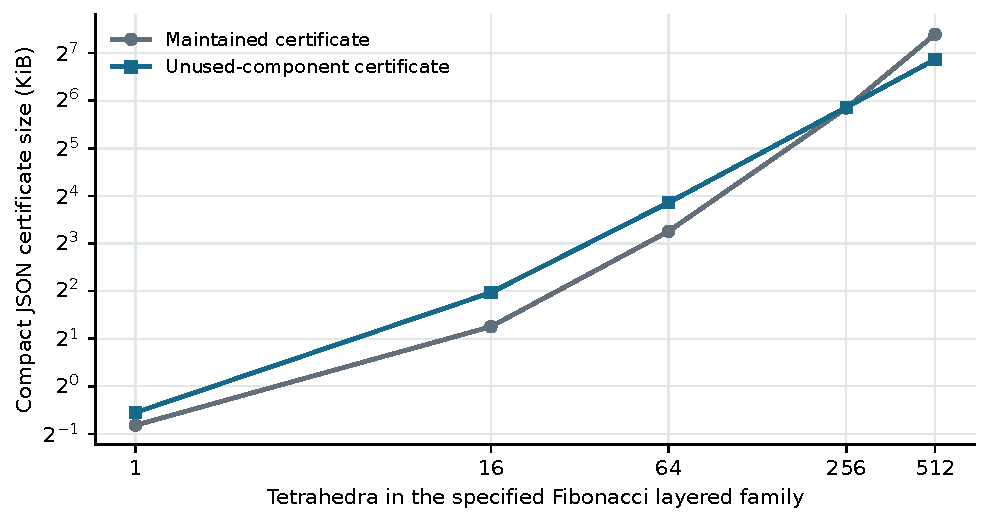
\includegraphics[width=.84\linewidth]{figures/certificate_sizes.pdf}
\caption{Recorded compact-JSON certificate sizes on the specified
Fibonacci layered family.  Lines connect measured points only.  Small
instances expose the new format's overhead; the proof of its asymptotic
advantage is Proposition~\ref{prop:unused-fibonacci-separation}, not a
fit to this plot.}
\label{fig:certificate-sizes}
\end{figure}

The graph experiment isolates the cost of retaining source provenance
while shrinking the operational graph.  Its realizable examples contain
three solid-torus-type vertices and an increasingly long chain of ball-type
vertices.  The kernel always has three vertices and two edges; the
certificate retains the full source-parent forest.

\begin{table}[htbp]
\centering\small
\begin{tabular}{rrrrr}
\toprule
Source vertices & Kernel vertices/edges & Production, ms & Replay, ms & Proof bytes\\
\midrule
10 & 3/2 & 0.034 & 0.044 & 593\\
100 & 3/2 & 0.252 & 0.335 & 2531\\
1000 & 3/2 & 3.003 & 3.499 & 26879\\
10000 & 3/2 & 36.015 & 44.774 & 319877\\
\bottomrule
\end{tabular}
\caption{Graph-only genus-three kernels with full source provenance, seven repetitions. Geometric source authentication and disc-chart construction are excluded.}
\label{tab:attachment-kernel-times}
\end{table}


This experiment excludes construction or authentication of the vertex
manifolds and their disc charts.  It measures the graph routine described
in its theorem, not a hidden geometric ball-recognition algorithm.

\subsection{Package layout and replay}

The principal executable interfaces are as follows.

\begin{description}[style=nextline]
\item[\code{decompose\_unused\_handles}]
Consumes a validated raw torus-boundary source.  Returns a geometric
decomposition and a numerical case, with no irreducibility assertion.
\code{verify\_unused\_handle\_certificate} reconstructs source cells and
replays the trace independently.
\item[\code{compile\_diagram\_initial\_core}]
Consumes a classical knot diagram and derives its canonical exterior.
Its checked outputs are \code{UNKNOT}, \code{ADMISSIBLE\_CORE}, or
resource-limited \code{INCONCLUSIVE}.  The independent wrapper checks
the exact diagram and exterior provenance before using the genus theorem.
\item[\code{kernel\_from\_decomposition}]
Converts the source decomposition format into a rooted-forest graph
certificate.  It is an adapter, not a substitute for the geometric
checker.  The independent graph checker accepts the original Euler labels
and edge incidences alongside the proposed certificate.
\item[\code{normal\_parallelity\_moment\_words}]
Consumes a triangulation and binary normal coordinates, and returns the
complete native cyclic interface with exact lengths.  The independent
checker rebuilds the source through the reference path.  The optional
\code{moments\_from\_parallelity\_packet} entry point additionally verifies
and retains a complete upstream parallelity certificate.
\end{description}

From the archive root, the following commands run the complete delivered
suite and small verified examples:
\begin{lstlisting}[language=bash]
python3 -m pip install -r requirements.txt
python3 run_checks.py
python3 examples.py
\end{lstlisting}
The test runner inserts the new code and pinned native snapshot into its
import path.  The examples show a positive unknot certificate, the
intermediate trefoil core, and an exact native boundary query.  Representative
native certificates can also be replayed without running discovery, using
\code{code/native\_moments\_replay.py} with the import path documented
in the root README.

The new algorithms use Python's standard library.  Regina 7.4 is listed
to reproduce the separate topology controls in the complete recorded run.
Matplotlib is needed only to regenerate the figures, which are already
included.  A TeX distribution builds the article using
\code{latexmk -pdf hierarchy\_primitives.tex} from its article directory.
No private external data source is needed for reproduction.

\subsection{Suggested repository integration}

The initial integration should preserve the package as an additive
research contribution, with its exact source revision and evidence.
\code{integration/INTEGRATION.md} maps the modules to a proposed maintained
placement and records the private source APIs they currently use.
The pinned source snapshot is for reproduction; an integrated tree should
use the repository's matching maintained modules instead of maintaining a
second copy of them.

For a first opt-in recognizer change, call the canonical-diagram initial
compiler at the same stage as the existing source-handle operator.
Accept a positive result only through the diagram-bound checker.  A
returned core should enter the next stage only once that stage supports
the inherited handle presentation and its normal-coordinate interface.
For the boundary compiler, compare full old and new outputs in a
differential integration mode, then select the new operator only under
its documented source contract.  Preserve caps and interruption behavior.

No default dispatch or remote repository mutation is included in this
deliverable.  The package supplies concrete code and proofs for review;
the unresolved patterned and global interfaces remain explicit research
tasks.  The goal of the proposed integration is to reduce real local work
while keeping every eventual recognition claim attached to its geometric
authority and complete complexity accounting.


\clearpage
\bibliographystyle{plainnat}
\bibliography{literature-references,repository-references}
\end{document}
